% to choose your degree
% please un-comment just one of the following
\documentclass[bsc,frontabs,twoside,singlespacing,parskip,deptreport]{infthesis}     % for BSc, BEng etc.
% \documentclass[minf,frontabs,twoside,singlespacing,parskip,deptreport]{infthesis}  % for MInf

\usepackage{graphicx}
\usepackage{wrapfig}
\usepackage{amsmath}
\usepackage{float}
\usepackage[round]{natbib}
\usepackage{listings}
\usepackage[dvipsnames]{xcolor}
\usepackage{subcaption}
\usepackage[title]{appendix}
\usepackage{verbatim}

\usepackage{minted}

\graphicspath{ {images/} }

\begin{document}

\title{Memory through key-value stores}

\author{Mantas Serapinas}

% to choose your course
% please un-comment just one of the following
%\course{Artificial Intelligence and Computer Science}
%\course{Artificial Intelligence and Software Engineering}
%\course{Artificial Intelligence and Mathematics}
%\course{Artificial Intelligence and Psychology }   
%\course{Artificial Intelligence with Psychology }   
%\course{Linguistics and Artificial Intelligence}    
\course{Computer Science}
%\course{Software Engineering}
%\course{Computer Science and Electronics}    
%\course{Electronics and Software Engineering}    
%\course{Computer Science and Management Science}    
%\course{Computer Science and Mathematics}
%\course{Computer Science and Physics}  
%\course{Computer Science and Statistics}    

% to choose your report type
% please un-comment just one of the following
\project{Undergraduate Dissertation} % CS&E, E&SE, AI&L
%\project{Undergraduate Thesis} % AI%Psy
\project{4th Year Project Report}

\date{\today}

\abstract{
Sometimes people come across programs, which cannot fit into main memory. This project proposes a software solution aimed to run a user program using key-value cloud storage service, which provides huge amounts of memory, as the main memory source. The implemented translation tool changes all store and load instructions to put and get operations on Google Bigtable storage using LLVM transformation pass with its \texttt{opt} tool. After noticing that virtual memory was still being allocated on heap allocation function calls, two custom heap allocators were implemented: first-fit free-list and the one without freed memory re-usage. The benchmarking results showed that the allocator without freed memory re-usage works significantly faster than both first-fit free-list and the default allocators. The implementation of a custom heap allocator was  advantageous as it made it possible to create a heap memory translator, which only translates store and load instructions operating on heap memory. The programs instrumented by heap translation tool work faster but have a huge overhead on the instruction count. Overall, the translated programs work orders of magnitude times slower but some solutions to alleviate this problem were identified.
}

\maketitle

\section*{Acknowledgements}

I would like to express my gratitude to my supervisor Vijay Nagarajan for aspiring guidance and advice.

I would also like to thank Harry Wagstaff and Aaron Smith for invaluable advice.

Finally, to my family and friends for their support and encouragement.

\tableofcontents

\pagenumbering{arabic}


\chapter{Introduction}

\section{Motivation}

Many computing applications demand a large amount of memory space. All this memory has to be provided by the primary memory, also called random access memory (RAM). On some operating systems (i.e. Linux or Mac OS), when the primary memory fills up and more memory is needed for a process, the operating system moves inactive pages in memory to a swap space. Swap space is an area of disk set aside to store data not immediately required in memory. While swap space can help machines with a small amount of RAM, it is limited and might not be enough to fulfil program's memory requests. Some systems have hard limits on the amount of memory a process can operate on and thus deny any excessive amounts of memory allocations. Other systems behave more wildly, allowing to allocate more memory than the system has and eventually starts killing processes by some predefined heuristic \citep{run_out_of_mem}. Neither of the strategies solves the problem of main memory shortage and the only possible solution seems to be physically adding more RAM to the system. This project proposes a software solution aimed to run a user program using key-value cloud storage as the main memory source.

The decision to use key-value cloud storage was based on the progress cloud services made during the last decade. We are particularly interested in NoSQL data stores \citep{nosql-data-stores}. NoSQL can be completely schema-free, with most popular data models being key-value stores, document stores, column-family stores, and graph databases. It is able to scale horizontally over many commodity servers, thus providing huge amounts of memory storage. Some cloud storage services (i.e. Google Bigtable) even provide in-memory tables, which greatly decreases read and write times in such systems.  On top of that, some cloud data management systems provide strong consistency model, which means that after an update operation all nodes agree on the new value before making it available to the user. All these properties let cloud storages be used as the main memory source.

The proposed solution in this project is somewhat similar to the idea of network RAM. When using network RAM, the system pages to idle memory over the network rather than to disk. This seems like a valid solution from the performance perspective, as the latency of some networks is much lower than the latency of disk seek \citep{numbers_should_know}. Although the main purposes of using such systems are described to be performance improvement \citep{Anderson:1998:ENR:893677} and better resource utilisation in distributed systems \citep{1327942}, it can also benefit as an external memory provider. For our project, the cloud storage stands as an abstraction of parallel network RAM. However, as the concept of a network RAM was discovered in one of the final stages of project development, the proposed solution uses the network RAM (or the cloud storage) as substitution not only for the disk but also for main memory accesses. This, of course, makes the instrumented programs very inefficient and is identified as one of the key improvements for future work.

The solutions on how to expose cloud storage as the main memory source, their advantages and disadvantages were identified:

\begin{itemize}
\item
\textbf{Explicit management by user.} This solution requires the user to explicitly move data back and forth from either disk or cloud storage using an API to store and retrieve values from cloud storage. It requires a lot of code modification, thus might not be well accepted by users.
\item
\textbf{Compiler}. This solution compiles the user code with an implemented compiler. The compiler would use cloud storage API to get and put values instead of using store and load instructions. The solution doesn't require any source code modification. However, this solution is not portable with different languages and seems too excessive and unrealistic given the timespan of the project.
\item
\textbf{Program transformation (LLVM)}. This solution involves compiling the user source code to LLVM IR and passing it through an implemented transformation pass, which translates all store and load instructions to get and put operations on the chosen cloud storage. This solution is more portable as it works will all languages, which have LLVM frontend, and all architectures supported by LLVM.
\item
\textbf{Binary translation}. This solution involves translating machine code from one instruction set architecture to another and is best used when source code is not available. Binary translation is further split into:
\subitem
\textbf{Static}. Static binary translation transforms the machine code to work on the target architecture without having to run the code. This approach is more efficient than dynamic binary translation. However, it is not a complete solution, due to problems such as dynamic linking and self-modifying code.
\subitem
\textbf{Dynamic}. Dynamic binary translation transforms the code on the fly by looking at the upcoming instructions, translating and caching them any further reference. The translation during runtime incurs a significant overhead but can be amortised when translated instructions are executed multiple times.
\end{itemize}

After careful examination, it was decided to implement a program transformation solution using LLVM tools and compiler. It is one of the most portable solutions, incurs only a minimal overhead during program's runtime (due to increased instruction count) and does not require any modification to the source code, as the transformation is done during the compilation. Moreover, it is assumed that the source code of the program exists, thus eliminating the need of binary translation.

\section{Scope}

It was understood that an industry quality tool should be as portable as possible and work with any cloud storage. However, due to the limited timespan of the project, it was decided to create a modular proof of concept tool that works with Google Bigtable and could be easily extended to work with other cloud storages. For the same reason, the implemented tool works only with programs written in C and C++. These specific languages were selected as they are both fully supported by LLVM through Clang compiler, while other languages are mainly supported by LLVM community created compiler frontends.

\section{Contributions}

The contributions of this paper are as follows:
\begin{itemize}
\item
Research and benchmark of multiple Google data stores.
\item
Implementated the tool which translates all program's load and store instructions to get and put calls on Bigtable.
\item
Implemented two custom heap allocator: first-fit free-list and the one with no freed memory re-usage.
\item
Implemented a variant of the translation tool which instruments only the load and store instructions operating on heap memory.
\end{itemize}

\section{Synopsis}

Chapter 2 presents the main requirements for the data stores to be used as the main memory source. The chapter continues with the discussion about the results of the benchmark ran on three Google cloud data-serving systems, namely Bigtable, Datastore and Spanner, followed by a more in-depth look at the chosen system, Bigtable. Finally, the chapter introduces the three functions implemented to read and write the contents of Bigtable.

Chapter 3 introduces LLVM project, gives a higher level picture of the translation tool followed by a more in-depth look at the implementation of the tool. Finally, the chapter ends with the issues encountered during translation tool development.

Chapter 4 presents the virtual memory waste problem, introduced by storing heap variables on Bigtable, and describes the solution - custom heap memory allocator. Two heap allocators are introduced: first-fit free-list and the allocator without freed memory re-usage. Finally, the chapter discusses the consistency of the proposed allocators on multithreaded applications and finishes with virtual memory usage and performance analysis.

Chapter 5 introduces the implemented heap memory translation tool, which only translates load and store instructions operating on heap memory space.

Chapter 6 presents the evaluation of the two translation tools based on the performance and instruction count of the programs.

Chapter 7 summarizes the work done and proposes a few possible improvements for future work.

\chapter{Data store}

\section{Overview}

The proposed translation tool instruments the program and makes it use the cloud data store as the main memory source. For the purpose of the project, a single cloud storage solution was chosen.
The main requirements for the data store were:

\begin{itemize}
\item
provide high throughput and low latency read and write operations;
\item
provide strong consistency model;
\item
provide a geographical locality for the machine that runs the instrumented program and the data store. In other words, have an option to choose that both machines would be located in the same data centre. This provides better throughput and latency results, as the nodes in the same data centre have very high bandwidth (1 Gbps - 100 Gbps) connections;
\item
provide a C++ API for data store operations;
\item
preferably provide key-value database model.
\end{itemize}

After a brief research three Google cloud storages were selected for further examination: Bigtable, Datastore and Spanner. Even though neither of the three candidates has a key-value store as their primary database model, they are one of the few that provide a C++ API for data store operations. This is achieved by using a combination of gRPC and protobuf libraries and Google APIs. Furthermore, all of the three storages have an option to be located in the same data centre as the machine running the instrumented program. All of the three data stores provide strong consistency models, with Spanner providing an even stronger model, namely external consistency\footnote{External consistency guarantees that for any two transactions, T\textsubscript{1} and T\textsubscript{2}: if T\textsubscript{2} starts to commit after T\textsubscript{1} finishes committing, then the timestamp for T\textsubscript{2} is greater than the timestamp for T\textsubscript{1}.}. Finally, the three selected Google data-serving systems were further analysed by performing a benchmark for their throughput and latency results.

\section{Benchmarking results}

The benchmarking was done using Yahoo! Cloud Serving Benchmark(YCSB) \citep{ycsb} tool. YCSB is an open-source framework for evaluating and comparing the performance of multiple types of data-serving systems. A key feature of YCSB, as described by its developers and users, is its extensibility, as it supports easy definitions of new systems and workloads. Workloads define the data that is loaded into the data store during the loading phase, and the operations are executed against the data set during the transaction phase. Workloads allow to better understand the performance tradeoffs of different data-serving systems.

The main operations done by the program instrumented with the translation tool are reads and writes with a small amount of read-modify-write for possible atomic operations. The predefined workloads A (update heavy) and F (read-modify-write) were selected out of six provided by YCSB framework, as they correctly imitate the behaviour of an average user program. 

For the best results, the benchmark was run on Google Compute Engine (GCE) virtual machine situated at the same data centre as the data stores.

The benchmark consists of two phases: loading and transaction. In the loading phase, 1000 entries are inserted into each data-serving system. Figures \ref{fig:insert_operations}a and \ref{fig:insert_operations}b show the latency and throughput achieved by each cloud storage. The results show that both Bigtable and Spanner have much lower latency and higher throughput than Datastore. This might be due to the fact that Datastore, unlike the other to data-serving systems in question, is using synchronous replication, which makes the host wait until all replications are created, as described in Margaret's Rouse article Synchronous replication \citep{synchronous-replication}.

\begin{figure}[H]
    \centering
    \begin{subfigure}{.45\linewidth}
    	\centering
    	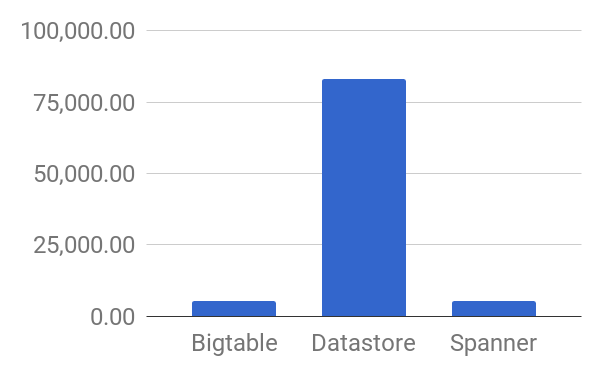
\includegraphics[width=6.5cm]{images/load-latency}
	\caption{Latency (\( \mu s\))}
    \end{subfigure}
    \hskip2em
    \begin{subfigure}{.45\linewidth}
    	\centering
    	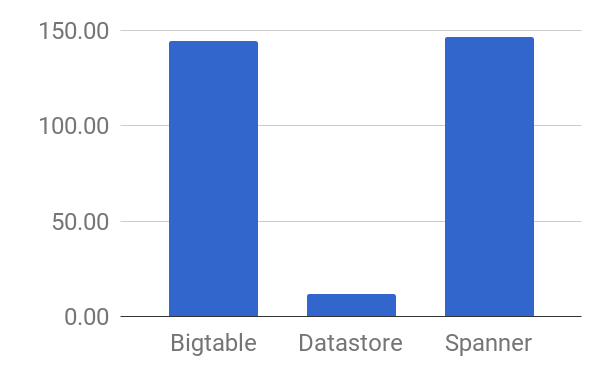
\includegraphics[width=6.5cm]{images/load-throughput}
	\caption{Throughput (\(ops/sec\))}
    \end{subfigure}
    \caption{Latency and throughput for 1000 insert (write) operations}
    \label{fig:insert_operations}
\end{figure}

In the transaction phase, two workloads were run. Workload A consists of 1000 operations (500 reads and 500 updates) while workload F consists of 2000 operations (1000 reads, 500 atomic read-modify-write operations and 500 updates). The results of the benchmark in terms of latency on write (update) operations were consistent with the previous loading benchmark results, with Bigtable and Spanner performing significantly better over Datastore (Figure \ref{write-latency}). However, the gap between Bigtable and Spanner was wider than the one observed in the loading phase, with Bigtable achieving the latencies of 4,627 \( \mu s\) on workload A and 4,682 \( \mu s\) on workload B, while Spanner struggling with the latencies of 9,944 \( \mu s\) and 7,338 \( \mu s\), respectively.

\begin{figure}[H]
	\centering
	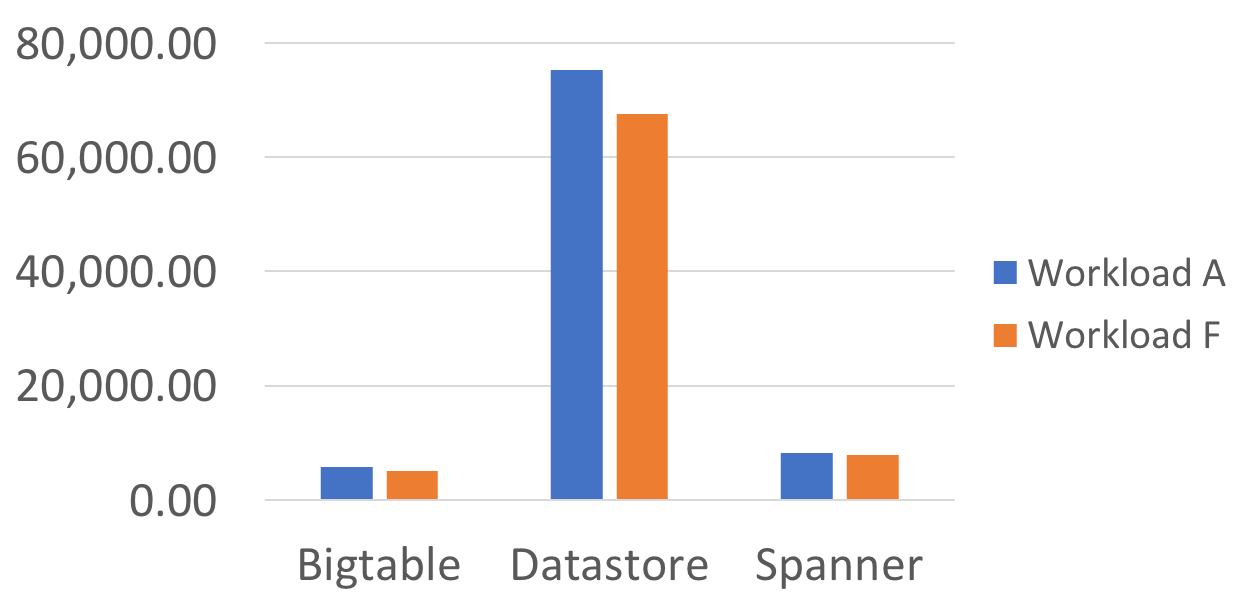
\includegraphics[width=12cm]{write-latency}
 	\caption{Update operations latencies (\( \mu s\)) for Workload A (500 writes) and Workload B (1000 writes)}
	\label{write-latency}
\end{figure}

Even though the difference on read operations latency between Datastore and two other data storages were smaller than with write operations (Figure \ref{read-latency}), Datastore still was more than two times slower than Spanner and more than 4 times slower than Bigtable. The latency results on read-modify-write operations showed a similar trend as read and write operations (Figure \ref{read-modify-write-latency}). 

\begin{figure}[H]
	\centering
	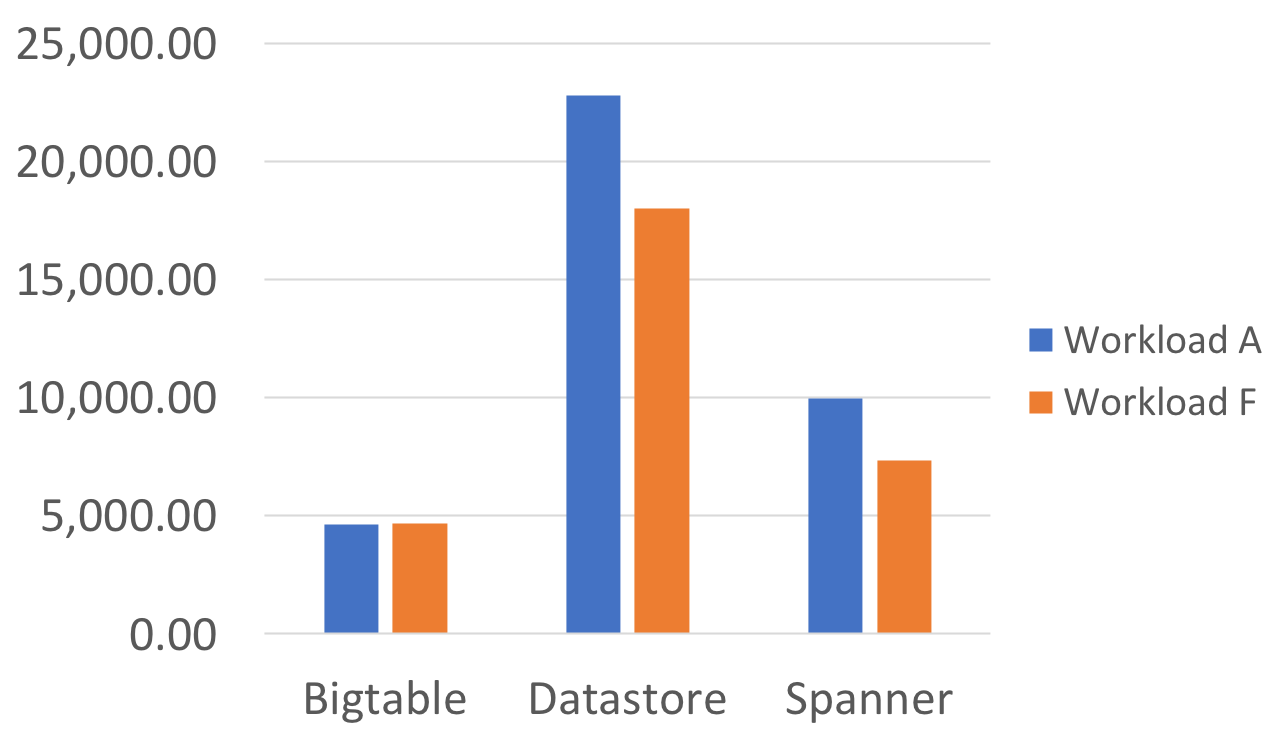
\includegraphics[width=12cm]{read-latency}
	\caption{Read operations latency (\( \mu s\)) for Workload A (500 reads) and Workload B (1000 reads)}
	\label{read-latency}
\end{figure}

\begin{figure}[H]
	\centering
	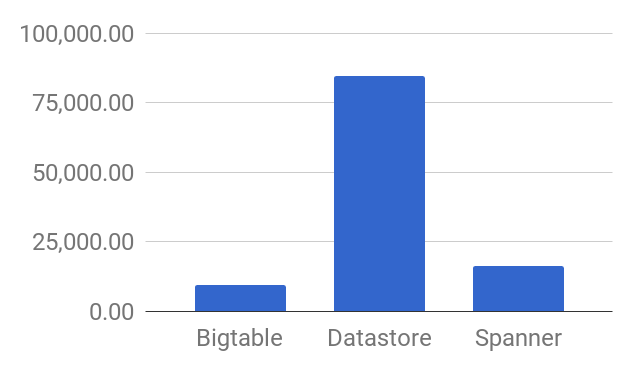
\includegraphics[width=12cm]{read-modify-write-latency}
	\caption{Read-modify-operations latency (\( \mu s\))}
	\label{read-modify-write-latency}
\end{figure}

The overall throughput for each workload, again, showed a significant superiority by Bigtable, as indicated in Figure \ref{throughput}. Bigtable achieved a throughput of 149.67 and 113.26 operations per second for workloads A and F, respectively. Spanner reached 105.63 and 78.19 operations per second, while Datastore performed worst with only 20.37 and 18.82 operations per second.

\begin{figure}[H]
	\centering
	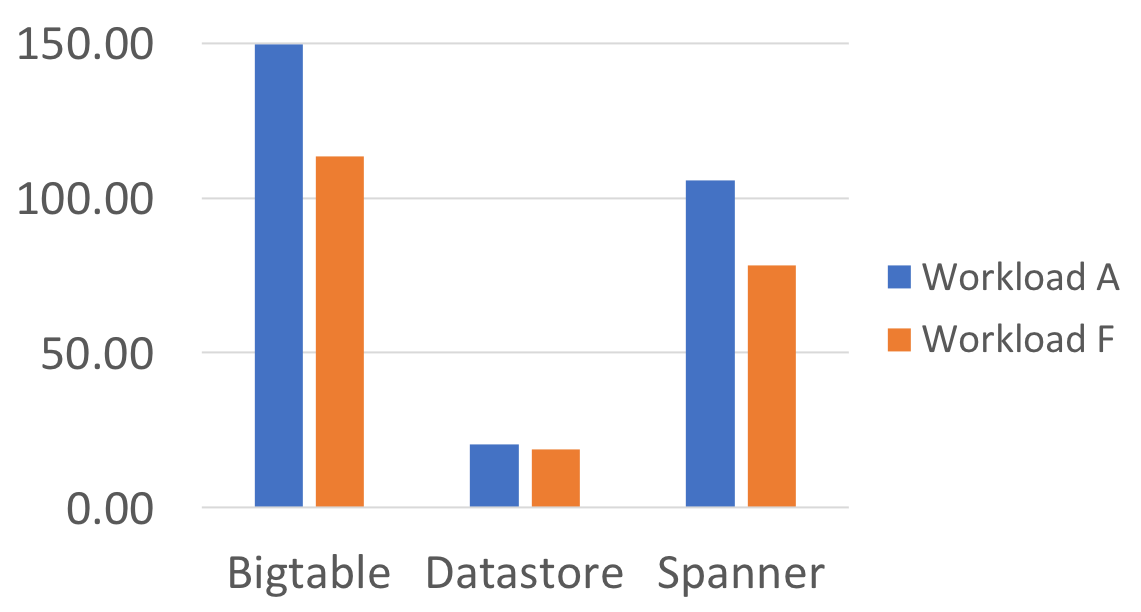
\includegraphics[width=12cm]{throughput}
	\caption{Throughput (\(ops/sec\)) for Workloads A (1000 operations) and Workload B (2000 operations)}
	\label{throughput}
\end{figure}

The benchmark proved Bigtable to be fastest among the three selected data stores. The latency results for write and read operations are similar to the ones provided in Google Cloud Platform Blog post introducing Bigtable \citep{bigtable-introduction}. Furthermore, the post claims Bigtable to provide cheaper write throughput (MB/s) per dollar performance than better read/write operations latency than their biggest competitors, namely HBase and Cassandra. Since Bigtable meet all the requirements set for data store and showed the best latency and throughput results, it was decided to use it as the main memory source for the programs instrumented with the translation tool. The next section gives a more in-depth look at Bigtable in order to better understand how it works and how it achieves such great performance.

\section{Bigtable}

Bigtable \citep{google-bigtable} is a high performance, wide column NoSQL database, designed to reliably scale to petabytes of data and thousands of machines. It is used by such Google products and projects like Google Analytics, Google Earth or Google Finance. Bigtable stores data in massively scalable tables, each of which is a persistent sorted key/value map. Tables consist of rows, each of which is essentially a collection of key/value entries, where the key is a combination of the column family, column qualifier and timestamp. Every read or write of data under a single row key is atomic. Moreover, Bigtable maintains data in lexicographic order by row key. The row range for a table is dynamically partitioned into tablets, which are the units of distribution and load balancing.

Bigtable uses the distributed Google File System (GFS) to store log and data files. It depends on a cluster management system for scheduling jobs, managing resources on shared machines, dealing with machine failures, and monitoring machine status. Bigtable data is stored using SSTable file format. Each SSTable contains a sequence of blocks. A block index is used to locate blocks; the index is loaded into memory when the SSTable is opened, allowing a lookup to be performed in a single disk seek. Optionally, an SSTable can be completely mapped into memory, which greatly increases the performance. However, such setup is very expensive and was not considered throughout the project.

Bigtable treats all data as raw byte strings. If a row does not include a value for a specific key, the key/value pair simply does not exist. Changes to a row take up extra storage space, as Bigtable stores mutations sequentially and compacts them only periodically.

Most importantly, Bigtable supports lookup value associated with the key operation and provides strong consistency - all writes are seen in the same order.

\section{Reading and writing the contents of Bigtable}

Bigtable uses gRPC client to read and write content using C++ remote function calls. According to gRPC webpage \citep{grpc}, gRPC client application can directly call methods on a server application on a different machine as if it was a local object (similarly to Java RMI). By default, gRPC uses protocol buffers, Google's open source language and platform neutral mechanism for serialising structured data. Figure \ref{fig:grpc} visualises communication between Bigtable and its gRPC clients (stubs). Bigtable gRPC client is provided through Google APIs repository. 

\begin{figure}[H]
\centering
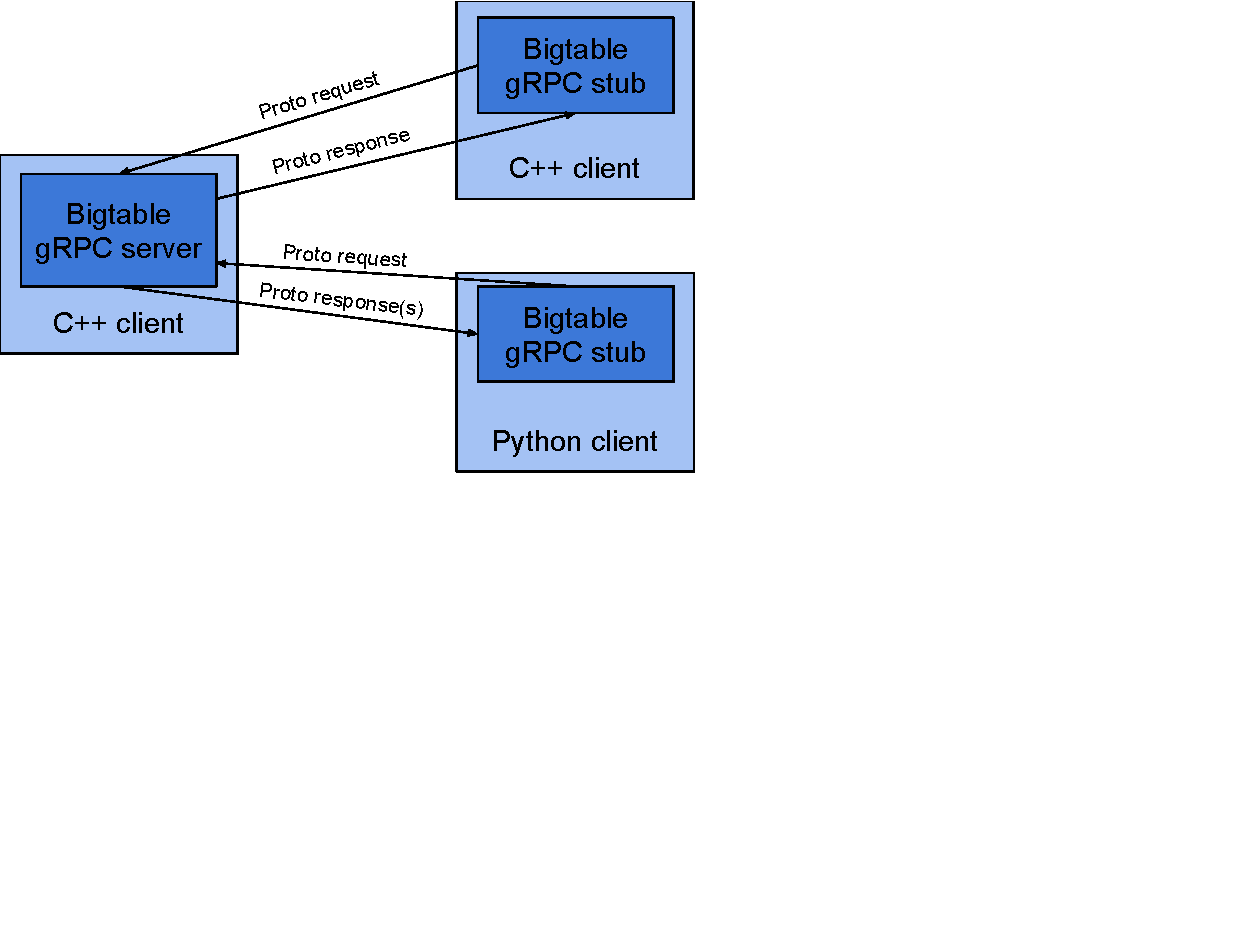
\includegraphics[width=0.55\textwidth]{images/grpc1}
\caption{Communication between Bigtable gRPC server and Bigtable gRPC stubs (clients)}
\label{fig:grpc}
\end{figure}

Get and put functions were implemented to abstract the specific details of the communication with Bigtable from the translation tool that calls them. This way the cloud storage service can be easily changed without the need to change the part that does the translation. 

\begin{listing}[H]
\begin{minted}[fontsize=\footnotesize]{c++}
void put(unsigned long long addr, long long val)  {
  // cast arguments to string type
  string address = std::to_string(addr);
  string value = std::to_string(val);
  // setup the request
  MutateRowRequest req;
  req.set_table_name(tableName);
  req.set_row_key(address);
  auto setCell = req.add_mutations()->mutable_set_cell();
  setCell->set_family_name(familyName);
  setCell->set_column_qualifier(columnQualifier);
  setCell->set_value(value);
  // invoke row mutation on Bigtable
  MutateRowResponse resp;
  grpc::ClientContext clientContext;
  auto status = bigtableStub->MutateRow(&clientContext, req, &resp);
}
\end{minted}
\caption{Writing content to Bigtable using put function}
\label{put}
\end{listing}

Put function takes two arguments, 64-bit integer as an address (key) and 64-bit integer as a value, and does not return anything (see Listing \ref{put}). First, the arguments are cast to string type. Then a new \texttt{MutateRowRequest} is built, by providing a full path to the table (including project, instance and table names), the row key, family name and column qualifier and value. Family name and column qualifier are constant as we are using Bigtable as key-value store, thus only one column family and qualifier are used. Finally, the \texttt{MutateRow} function is called remotely through Bigtable stub and response status is stored for debugging purposes.

\definecolor{codegreen}{rgb}{0,0.6,0}
\definecolor{codegray}{rgb}{0.5,0.5,0.5}
\definecolor{backcolour}{rgb}{0.95,0.95,0.92}
\lstset{
  mathescape=true,
  literate=
  	{->}{$\rightarrow{}$}{1}
}
\lstdefinestyle{block} {
  language=C++,
  backgroundcolor=\color{backcolour},   
  commentstyle=\color{codegreen},
  keywordstyle=\color{Maroon},
  numberstyle=\tiny\color{codegray},
  stringstyle=\color{magenta},
  basicstyle=\footnotesize,                 
  keepspaces=true,                                           
  tabsize=2,
  captionpos=b
}

Get function takes 64-bit integer representing the address (key) as an argument and returns a 64-bit integer value (see Listing \ref{get}). Similarly to put function, the address value is cast to string. A read row request is created by providing the full path to the table and address string is passed as a row key. The call on \texttt{ReadRows} function returns a stream, which is read by chunks and appended to the \texttt{valueStr} variable. The nested loops should run at most one time, as only one row key was provided. Before the value is returned, an if statement checks if the given key had the corresponding value in the table and if so, casts the value to 64-bit integer. If no value was found with corresponding key, the function returns 0. This behaviour is expected, when the program reads uninitialised variable.

\begin{listing}[H]
\begin{minted}[fontsize=\footnotesize]{c++}
long long get(unsigned long long addr) {
  // convert argument to string type
  string address = to_string(addr);
  // setup the request
  ReadRowsRequest req;
  req.set_table_name(tableName);
  req.mutable_rows()->add_row_keys(address);
  string valueStr;	
  // invoke row reading on Bigtable
  auto stream = bigtableStub->ReadRows(&clientContext, req);
    while (stream->Read(&resp)) {
      for (auto& cellChunk : *resp.mutable_chunks()) {
        if (cellChunk.value_size() > 0) {
          valueStr.reserve(cellChunk.value_size());
        }
        valueStr.append(cellChunk.value());
      }
    }
    // convert value to 64-bit integer
    long long value = 0;
    if (!valueStr.empty())
      value = stoll(valueStr);
    return value;
}
\end{minted}
\caption{Reading content from Bigtable using get function}
\label{get}
\end{listing}

Additionally, atomic increment function was implemented, which given an address and a 64-bit integer increment invokes Bigtable's \texttt{ReadModifyWriteRow} method with the \texttt{increment\_amount} rule. At first, the address is cast to string and set as a row key for \texttt{ReadModifyWriteRowRequest}. After request setup, read-modify-write operation is invoked. The respond message contains an array of bytes represented as an array of characters. A \texttt{bytesToInt} function was implemented in order to concatenate the bytes into a 64-bit value, which is then returned by the function.

\begin{listing}[H]
\begin{minted}[fontsize=\footnotesize]{c++}
long long atomic_increment(unsigned long long address, unsigned long long increment) {
  // convert address to string
  string address = to_string(address);
  // setup the request
  ReadModifyWriteRowRequest req;
  req.set_table_name(TABLE_NAME);
  req.set_row_key(address);
  ReadModifyWriteRule rule;
  rule.set_family_name(FAMILY_NAME);
  rule.set_column_qualifier(COLUMN_QUALIFIER);
  rule.set_increment_amount(increment);
  *req.add_rules() = std::move(rule);
  // invoke read-modify-write operation on Bigtable
  ReadModifyWriteRowResponse resp;
  grpc::ClientContext clientContext;
  auto status = bigtableStub->ReadModifyWriteRow(&clientContext, req, &resp);
  const char* bytes = resp.mutable_row()->mutable_families(0)->
  			mutable_columns(0)->mutable_cells(0)->value().c_str();
  long long value = bytesToInt(bytes);
  return value;
}
\end{minted}
\caption{A read-modify-write operation with an increment rule on Bigtable using atomic\_increment function}
\label{get}
\end{listing}

\section{Issues encountered}

Even though both gRPC and protobuf (protocol buffers) libraries are developed by Google, some difficulties were encountered while compiling source builds. The errors were made known to the developers \citep{grpc_issue}, but it has slightly stalled the development of the project.









\chapter{Translation tool}
\label{translation-tool}

The translation tool was implemented as a compiler level solution mainly because it makes the tool portable across different platforms and it doesn't require any user code modification. One possible way to implement a compiler level solution is by building a new compiler, which instead of using load and store instructions would call get and put functions on Bigtable. Of course, creating a new, industry-standard compiler would be too excessive and not feasible in the timespan of the project. Luckily, LLVM provides a compiler and lots of tools to instrument already compiled code.

\section{LLVM}

LLVM (Low Level Virtual Machine), began at the University of Illinois, is an open source compiler framework for building tools. It supports life-long program analysis and transformation for arbitrary programs. It has an industrial standard compiler (clang/clang++), which has an option to compile C/C++ code to an extensible, strongly typed intermediate representation, namely LLVM IR.

LLVM optimizing compiler, like other industry standard compilers, consists of several components: frontend, optimiser, backend and linker. The important advantage over other compilers is the use of LLVM Bitcode, which consists of a bitstream container format and an encoding of LLVM IR. It provides a clean API boundary separating the compiler frontend and backend, thus making it easier to swap in new frontend and backend components (Figure \ref{fig:llvm}). This is especially useful when developing a new language, as one only needs to create a new frontend component of the compiler and use the provided LLVM optimiser and backend components. 

Moreover, as LLVM project is open-source, users can create their own optimisation or transformation passes. Thus it is possible to create a transformation pass for \texttt{opt} tool, which would iterate over all of the RISC-like instruction set and translate load and store instructions to get and put function calls for Bigtable.

LLVM has lots of support and documentation on the Internet. Lots of well-known compilers, like NVIDIA's CUDA Compiler or Microsoft DirectX shader compiler, are based on LLVM. All of these features make LLVM a desirable framework to use for our translation tool.

\begin{figure}[H]
\centering
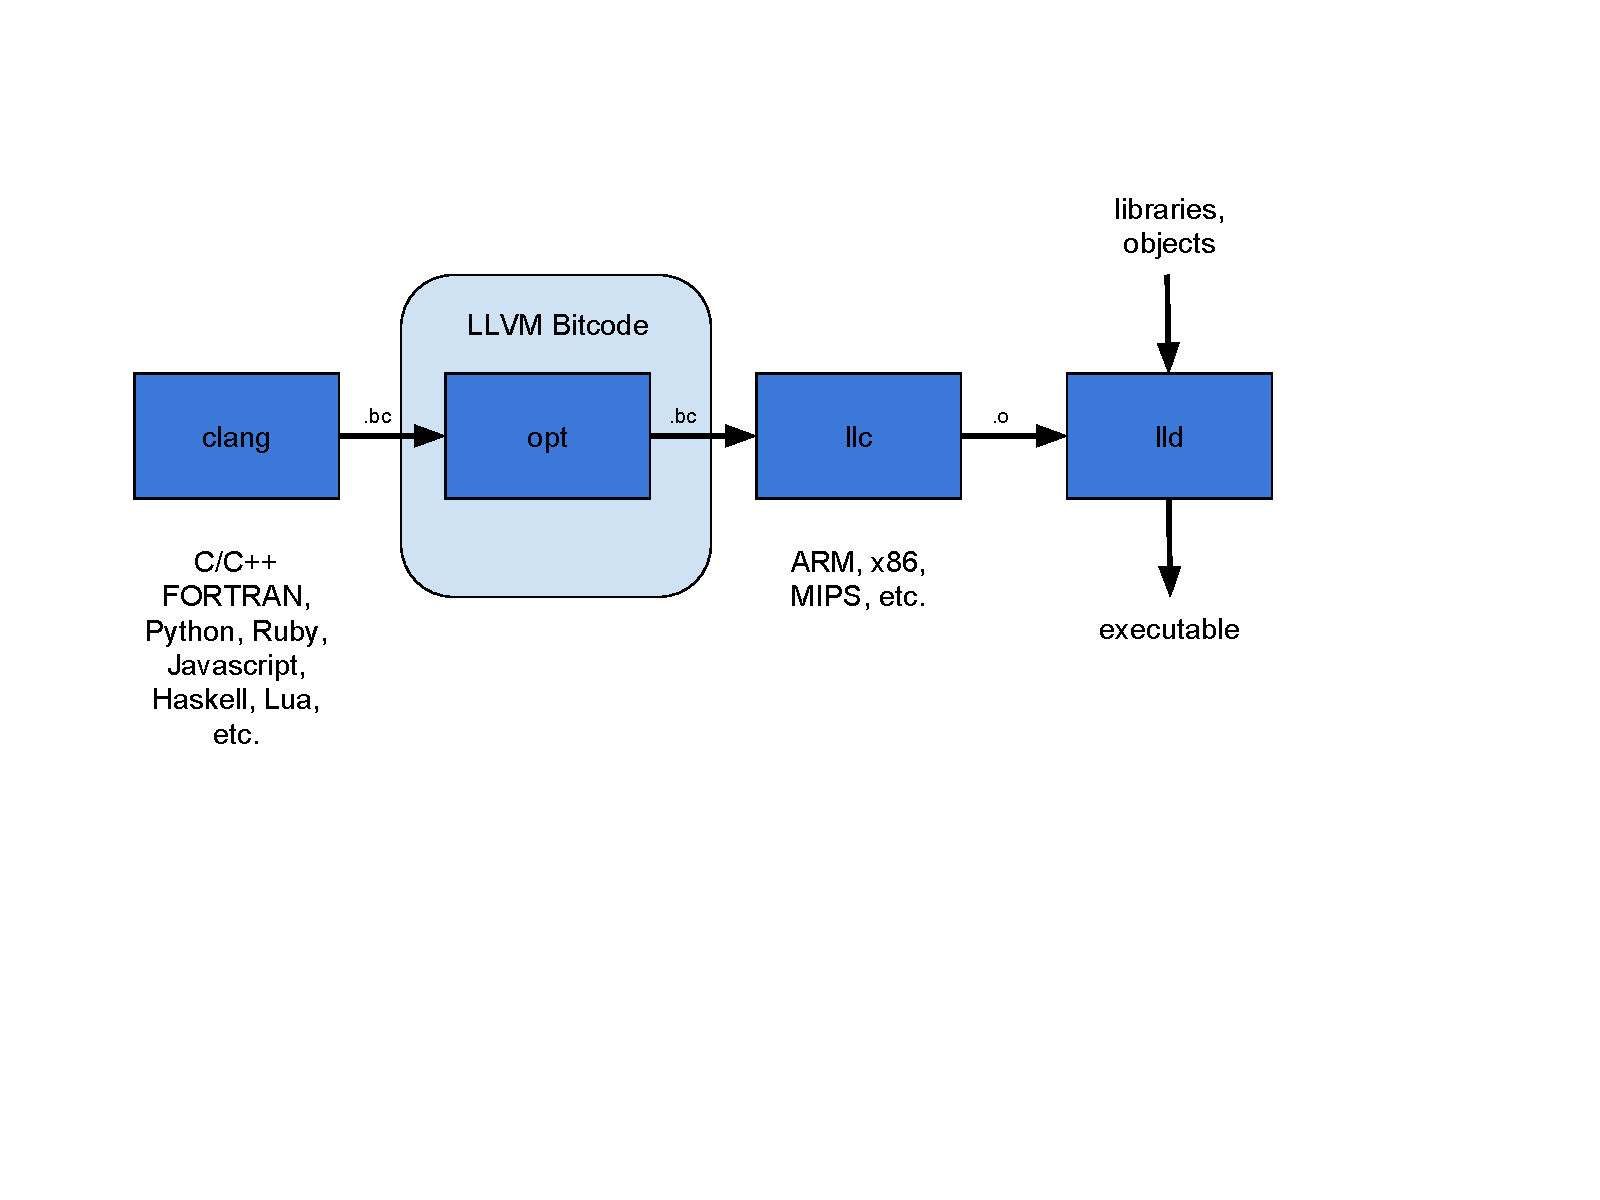
\includegraphics[width=1\textwidth]{images/llvm}
\caption{LLVM compiler architecture}
\label{fig:llvm}
\end{figure}

One problem encountered when working with LLVM is that it cannot get LLVM IR representation of C library functions, as C library located on the machine is already compiled and assembled. This introduces a problem, as C library functions use load and store instructions to retrieve the data from the main memory, which after our translation is done will be stored in the cloud storage. The solution is to use portable C libraries like \texttt{ulibc} or \texttt{newlib}. They are C libraries available in source form intended for use on embedded systems. These libraries can be compiled into LLVM IR code, thus letting the translation pass transform load and store instructions.

\section{Architecture}
\label{architecture}

The translation pass tool consists of 4 transitions (see Figure \ref{fig:architecture}). At first, user source code and Bigtable get and put functions are compiled to LLVM IR and combined into a single LLVM Bitcode file. As mentioned before, get and put functions of any other cloud storage could be used here. Additionally, any other C/C++ files which might be needed during the translation pass must be added at this stage. After that, the code is instrumented by our transformation pass using \texttt{opt} tool and is emitted with translated LLVM IR into the LLVM Bitcode file. Then the output is compiled into native machine code using \texttt{llc} tool and finally linked with gRPC, protobuf and any other linked libraries to build an executable.

\begin{figure}[H]
\centering
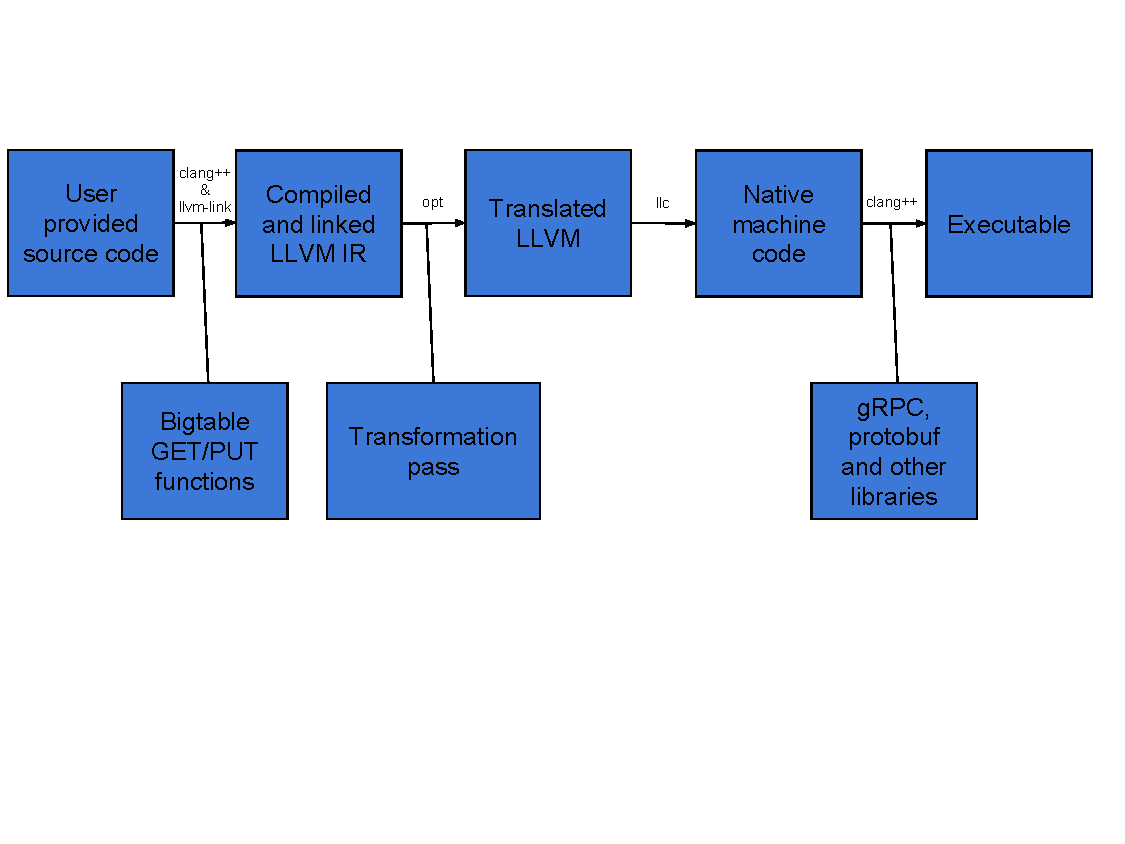
\includegraphics[width=1\textwidth]{images/architecture}
\caption{LLVM solution architecture}
\label{fig:architecture}
\end{figure}

After the first transition when user source code and Bigtable functions are compiled and combined into a single LLVM Bitcode file, the resulting LLVM IR consists of dozens of gRPC library functions. These functions must not be translated, as they are responsible for setting up the connection and invoking the methods on Bigtable. Thus, a barrier was added to the transformation pass, which stops the transformation when the first gRPC function is detected through the iteration. In order for this to work properly, the linking of LLVM Bitcode files in the first stage must be done in a strict order: Bigtable get and put functions file must appear after the code that must be translated\footnote{Notice that this implementation is only relevant for Google cloud storages. As other cloud services do not provide communication with storage using gRPC.}. This creates a barrier (see Figure \ref{fig:barrier}) between the code that is translated and the code which contains functions to be called by the translated code (i.e. put and get functions).

\begin{figure}[H]
\centering
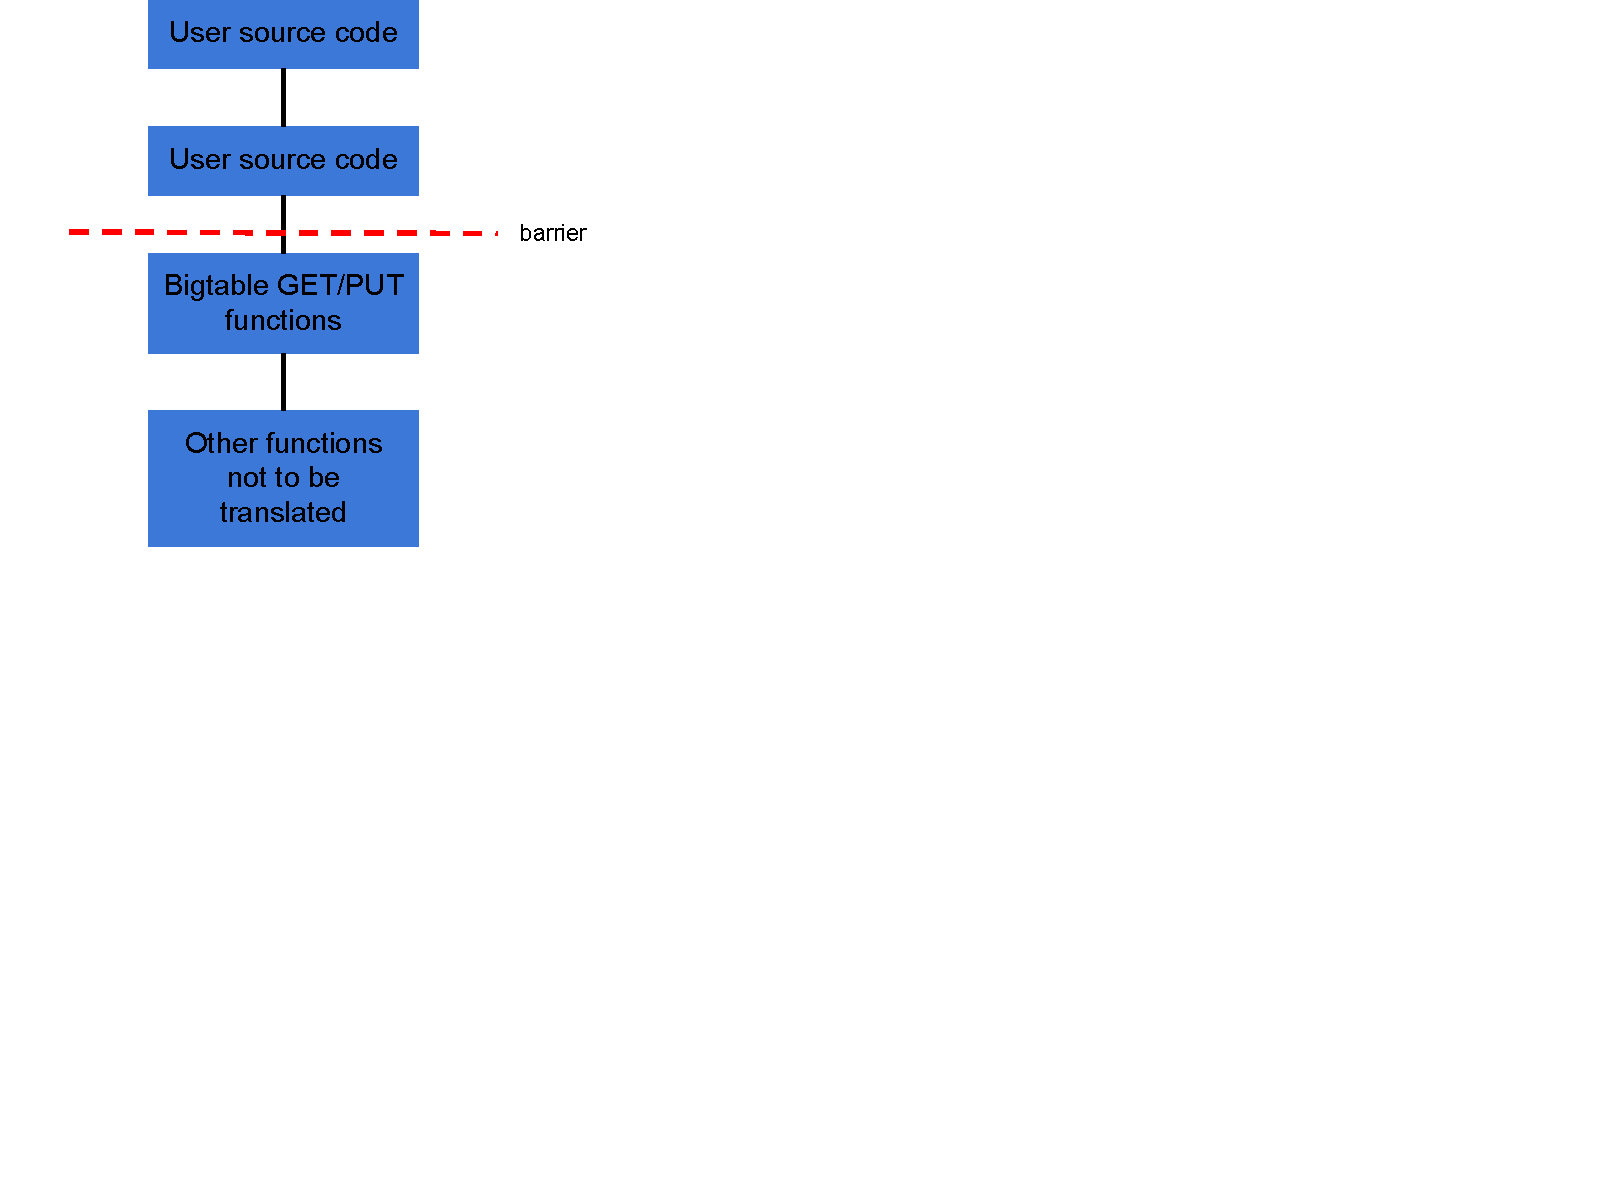
\includegraphics[width=0.5\textwidth]{images/barrier}
\caption{Translation barrier}
\label{fig:barrier}
\end{figure}


\section{Translation pass}

The previously mentioned barrier dividing instrumented and uninstrumented code is implemented by checking if the currently iterated function belongs to the original get and put functions file. The translation pass iterates over all instructions until the barrier. When the iteration reaches this function, the translation pass is ended.

Load and store instructions accept different types of arguments (remember, LLVM IR contains a strongly typed instruction set). For store instructions, the address must have a higher pointer indirection degree than the value. For instance, the corresponding store instruction for \mintinline{cpp}{int* x = &y} would have the address with the type of pointer to integer pointer (represented in LLVM as \mintinline{cpp}{**i32}) and the value with the type of integer pointer (\mintinline{cpp}{*i32}). For load instruction translations, get function must return the value of the same type as load instruction. 

The LLVM load and store instructions accept any types of values for their operands. The same functionality for get and put functions could be achieved by creating multiple overloads. However, this would mean creating numerous overloads for each single type in LLVM, as a new overload function would be needed for each pointer type with different indirection degree. For instance, get function which takes 32-bit integer pointer, would work with pointer to 32-bit integer pointer. For this reason, get and load functions only accept 64-bit integer arguments and depend on additional instructions to enforce this type. This makes the translation of store and load instructions more complicated than just replacing one instruction with the other.

\begin{figure}[H]
\centering
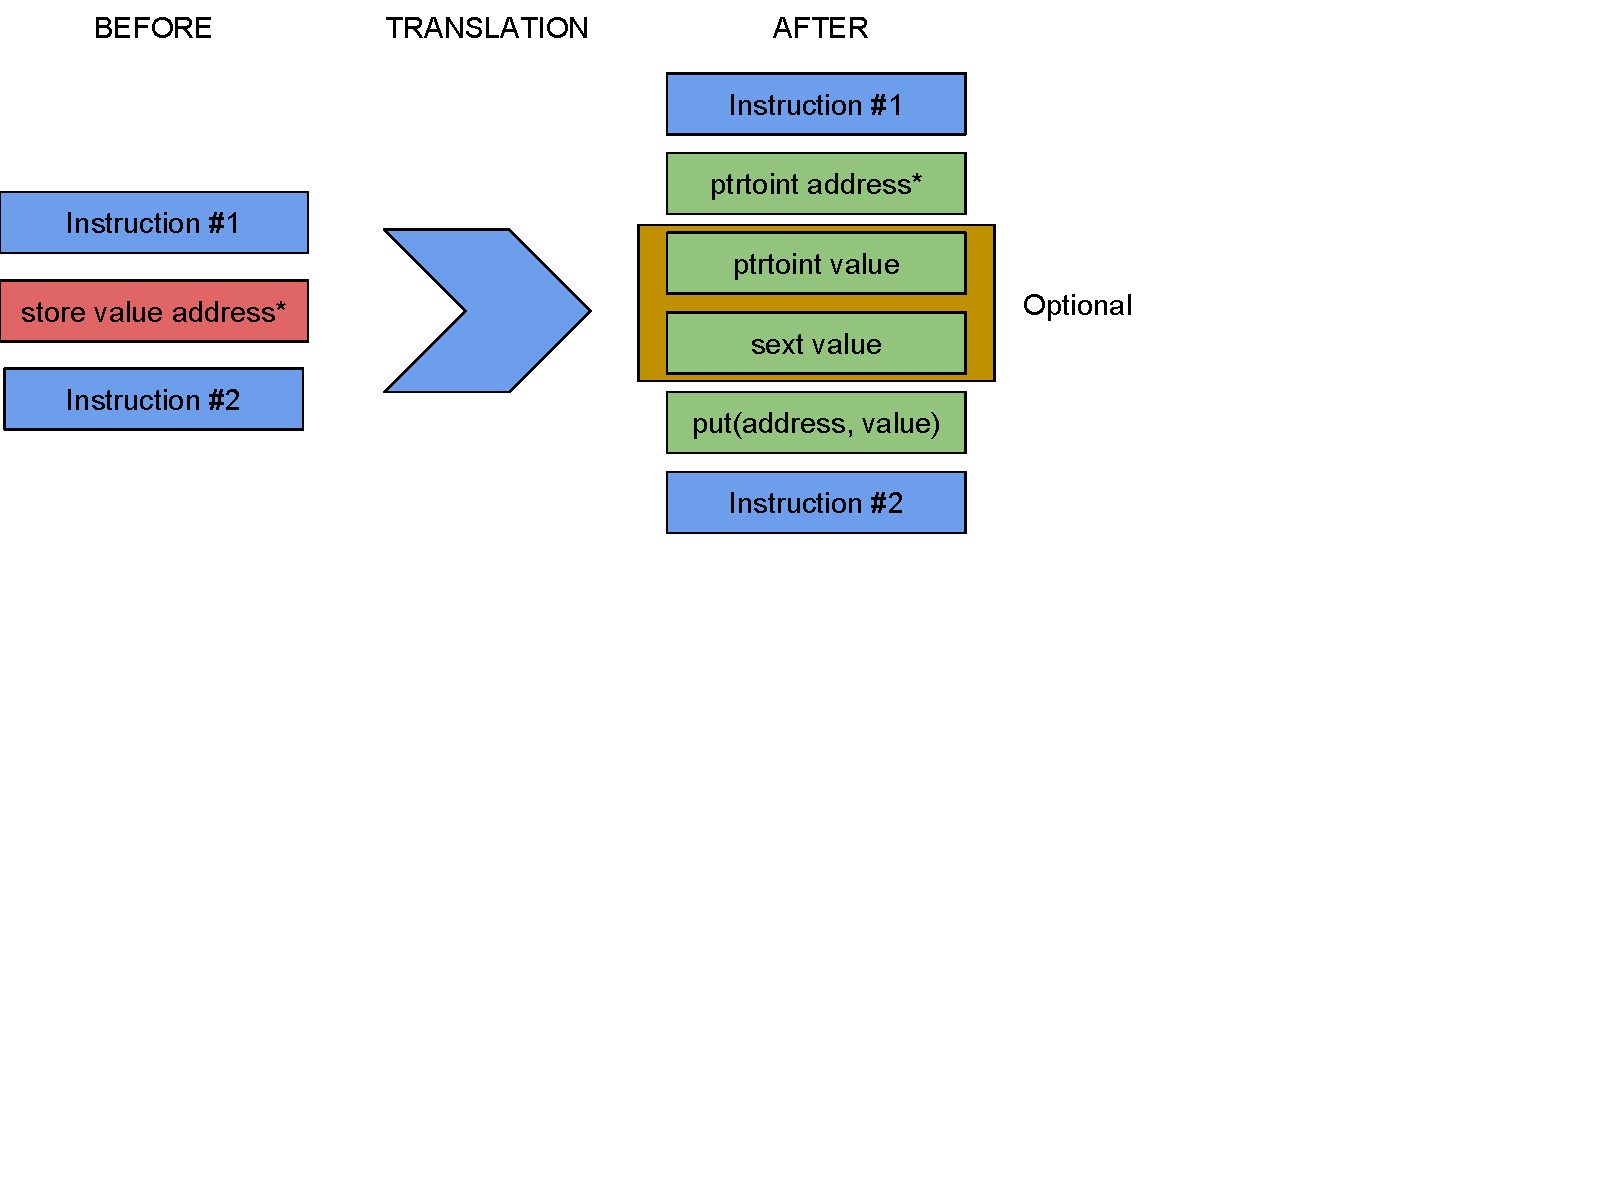
\includegraphics[width=0.8\textwidth]{images/store_translation}
\caption{LLVM instruction set before and after store instruction translation}
\label{fig:store_translation}
\end{figure}

Store to put instruction translation starts by converting the 64-bit integer pointer (address) with \texttt{ptrtoint} instruction. If the value is of integer type and not 64 bits wide, it is sign extended using \texttt{sext} instruction. If the value is of pointer type it is cast to 64-bit integer by \texttt{ptrtoinst} instruction. Otherwise, it is assumed to be 64-bit integer\footnote{Although it might be of some other type (i.e. struct). These types were not examined in the project and should be considered as future work.}. Finally, both arguments now being of 64-bit\footnote{64-bit integer type for get and put instruction arguments and/or return type was chosen deliberately. This is the maximum biggest type of integer, thus it makes the casting part a bit simpler. For example, if 32-bit integer type was chosen, some values would need to be sign extended while others would need to be truncated.} integer type are given as arguments to put function call. Figure \ref{fig:store_translation} shows a subset of the instruction set before and after store instruction translation.

Load instruction translation begins by identifying its return type and pointer indirection degree (only relevant if the value is of pointer type). Similarly to store translation, the address is cast to 64-bit integer using \texttt{ptrtoint} instruction and passed to get function as an argument. As the return type of get function is a 64-bit integer, it must be cast to the appropriate type (unless the load instruction actually returns a 64-bit integer). If the returned type is an integer, it is truncated to the expected integer bit width using \texttt{trunc} instruction. Finally, if the expected returned type is a pointer, the resulting value is converted to a pointer type with an appropriate pointer indirection degree (identified at the beginning) with \texttt{inttoptr} instruction. Figure \ref{fig:load_translation} shows a subset of the instruction set before and after store instruction translation.

\begin{figure}[H]
\centering
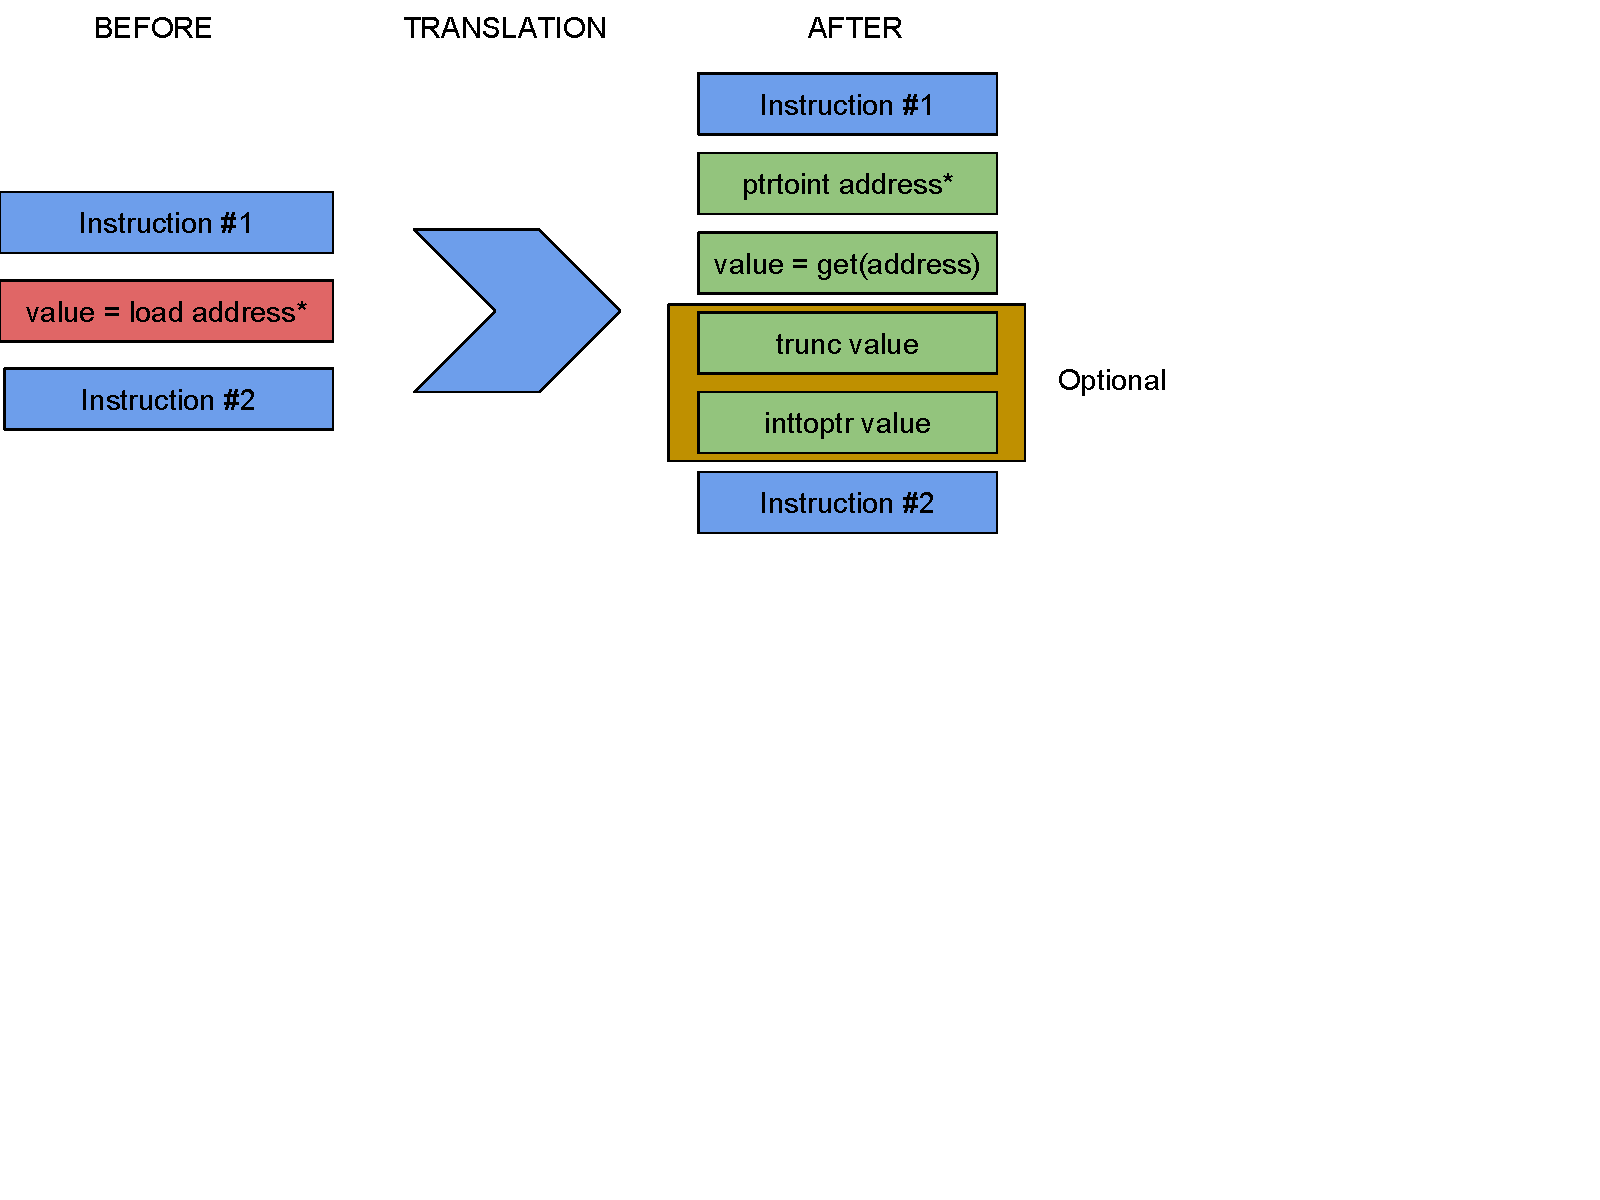
\includegraphics[width=0.8\textwidth]{images/load_translation}
\caption{LLVM instruction set before and after get instruction translation}
\label{fig:load_translation}
\end{figure}

\section{Other issues}
\label{section:other_issues}

As mentioned before, LLVM is a strongly typed system, consisting of 17 different types. On this project, the emphasis was given on the most commonly used types, namely integer type and pointer type. After implementing the translation pass and testing it with multi-threaded programs, it was discovered that a literal structure type was accessed using load instruction. Given the address to the structure, load instruction grabs the whole structure object as in memory it is stored as a contiguous block of memory. The problem arises when different element values to the structure are put on Bigtable in different rows. Thus, when load accessed the whole structure at once, our get function only gets the first element (or first row) of the structure object. The issue was remedied by identifying literal struct type load instructions, creating a \texttt{getelementptr} instruction for each structure element, getting the element values from Bigtable and inserting them all to the returned structure object. The translation of literal struct type load instruction is visualised in figure \ref{fig:struct_type}.

\begin{figure}[H]
\centering
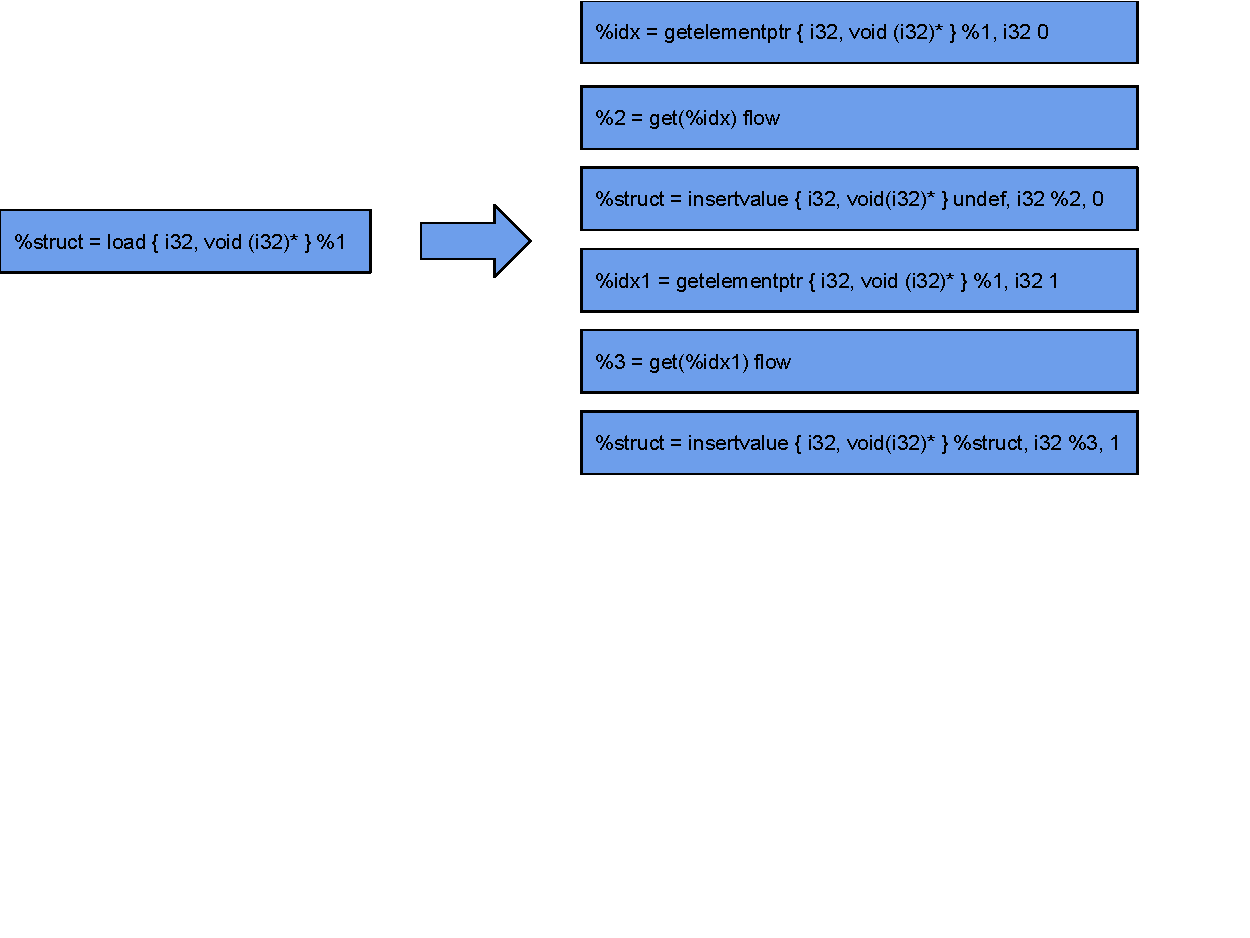
\includegraphics[width=0.8\textwidth]{images/struct_type}
\caption{Translation of literal struct type load instruction}
\label{fig:struct_type}
\end{figure}

However, even after implementing struct type load instruction translation, thread creation process with function arguments returns segmentation fault. The issue of the segmentation fault hasn't been discovered but it might be related to thread creation using OS functions, which expect the function arguments to be located in main memory. To deal with this problem, a filter was added to translation pass, which does not instrument thread creation functions. Any arguments that are being passed to thread function are being stored to main memory before thread creation process.

The translation tool doesn't cover all 17 LLVM types and together with thread creation issue are left as recommended future extensions and improvements.

\chapter{Custom heap allocator}

\section{Motivation}

Calls to malloc function allocate virtual memory space. When this allocated virtual memory is "touched" (i.e. loaded from or stored to), it is mapped to real memory by a call to a special function of the operating system (i.e. mmap). As translation tool eliminates all loads and stores to memory, the allocated memory is never accessed, thus never really mapped to physical memory. Nevertheless, the allocated memory is left unused on virtual address space. This might cause problems when a program tries to allocate more space than possible on virtual memory. Some operating systems (i.e. Windows or macOS) limit the virtual memory space, thus providing a custom heap allocator, which would reduce the amount of memory allocated on virtual address space, seems beneficial. Moreover, a custom heap allocator can be implemented to provide information about the allocated heap boundaries for the program. The reason why this might be advantageous is explained in Chapter \ref{heap-memory-translator}. 

\section{Implementation}

\subsection{First-fit free-list allocator}

One of the proposed solutions is a first-fit free-list heap allocator. The heap allocator implementation was based on Marwan Burelle's malloc tutorial \citep{malloc_tutorial} and adjusted to work on Bigtable. The heap allocator implements four functions: malloc, free, realloc and calloc. All of these functions are counterparts of the Standard C++ Library functions and have the same function definitions.

The allocator keeps a list of meta-data blocks, which contain information about chunks of data allocated with the new malloc. This lets the memory be reused after it has been released with a call to free function. Unlike in tutorial implementation, only meta-data objects are stored on the main memory. The actual requested space is allocated on Bigtable. Thus, the implemented custom heap allocator uses two heaps: main memory and Bigtable. Figure \ref{fig:heap_organisation} sketches the memory organisation of two heaps. The structure of meta-data blocks described in the tutorial were adjusted to reflect these changes. Besides storing the size of data block and pointers to other blocks, the meta-data blocks also store the address of data block on Bigtable.

\begin{figure}[H]
\centering
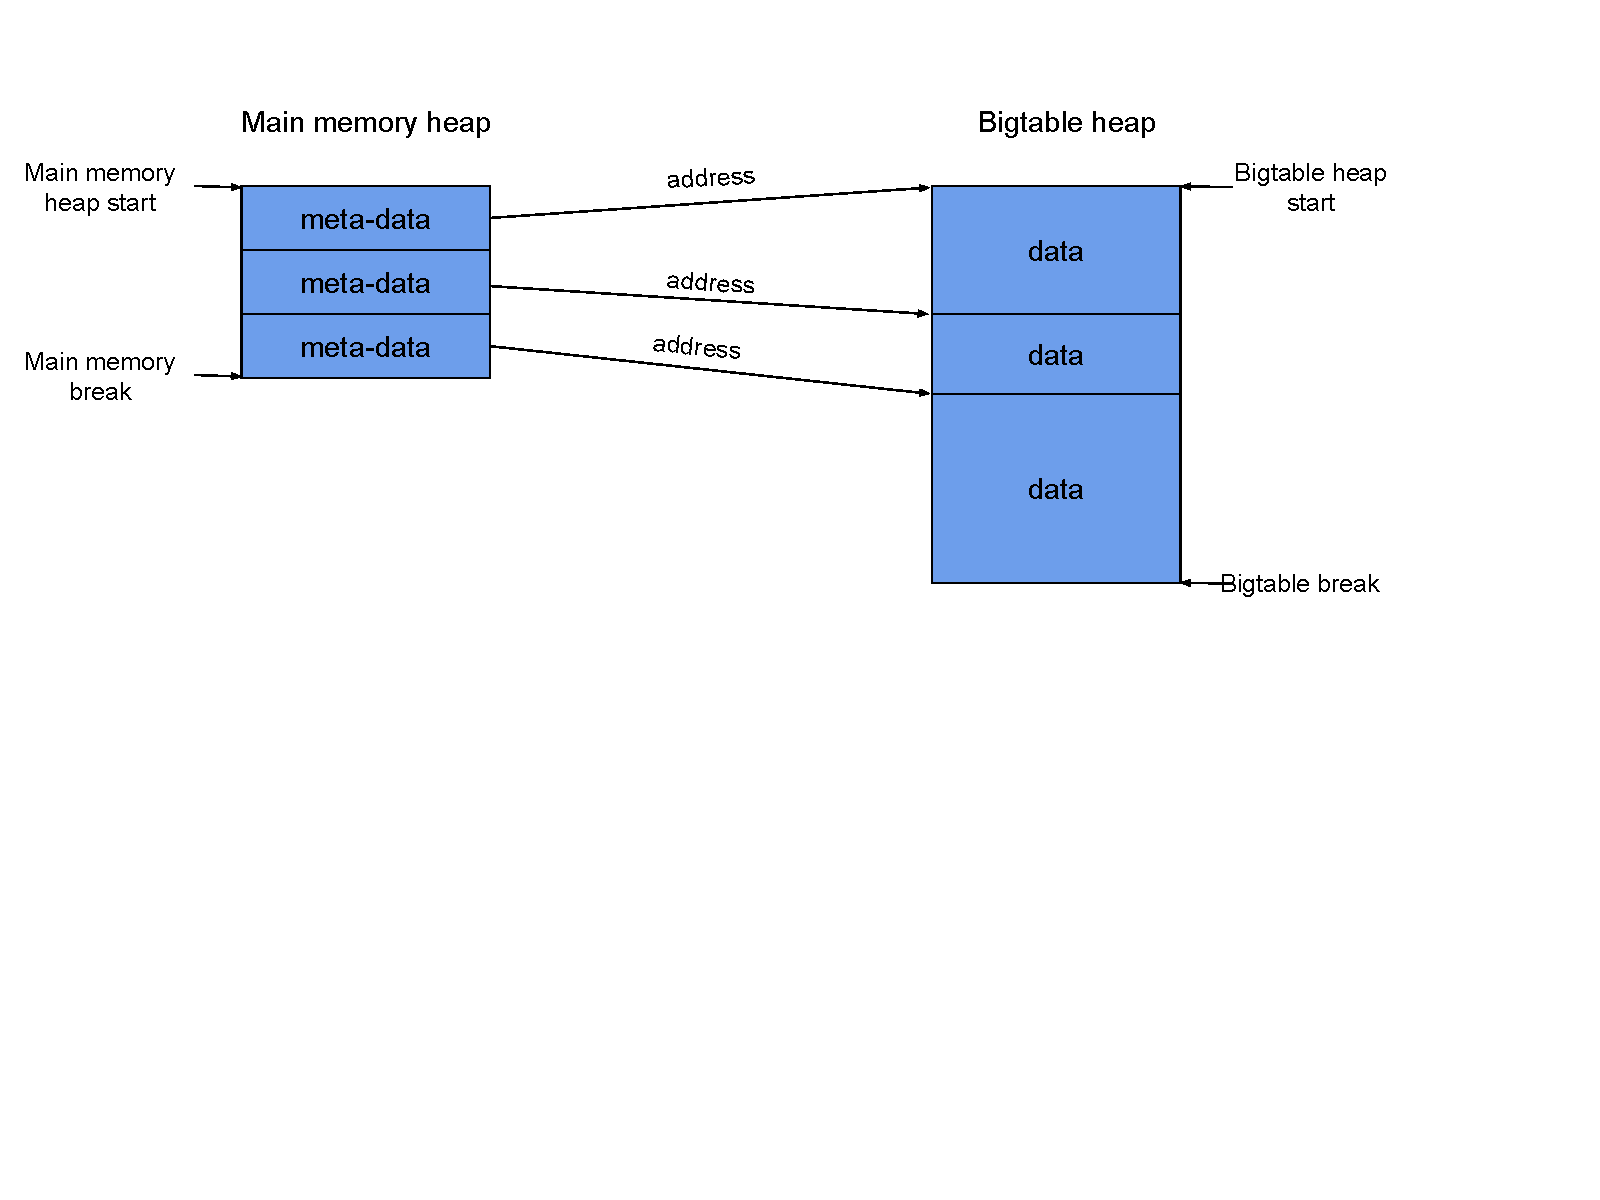
\includegraphics[width=1\textwidth]{images/heap_organisation}
\caption{Heap memory organisation using the proposed heap allocator}
\label{fig:heap_organisation}
\end{figure}

The main memory heap is managed by the default memory allocator (Standard C++ library provided malloc, free, etc). All of the malloc (and other memory allocation functions) calls in the user source code are translated to custom heap allocator function calls using the translation pass described in the previous chapter. Other memory allocation function calls (i.e. in gRPC functions) are not translated and use the default allocation functions.

The heap on Bigtable is implemented as a continuous space of memory with two bounds: the start of the heap and the endpoint  called the Bigtable break. The start of the heap is initialized on the first call on custom malloc function by calling \texttt{sbrk} function with an increment equal to 0 (this returns the break address on the main memory heap). Thus, the start addresses of main memory and Bigtable heap are identical. The end of the heap is managed by set\_bt\_brk function, which was implemented to reflect the behaviour of \texttt{sbrk} function (see Listing \ref{setbtbrk}).

\begin{listing}
\begin{minted}[fontsize=\footnotesize]{c++}
void* set_bt_brk(int incr) {
  // if uninitialised, set to sbrk(0)
  if (current_bt_break == 0) {
    current_bt_break = (uintptr_t) sbrk(0);
    initial_bt_break = current_bt_break;
  }
  uintptr_t old_break = current_bt_break;
  current_bt_break += incr;
  return (void*) old_break;
}
\end{minted}
\caption{set\_bt\_brk function implementation}
\label{setbtbrk}
\end{listing}

An alternative way to implement such heap allocator is to allocate both meta-data objects and the actual requested space on the Bigtable, but this would increase the communication costs with Bigtable. As meta-data objects only take up to 40 bytes (on a 64-bit system), the decision was made to store them locally.

Malloc function starts by changing the requested size to be a multiple of 4 to align the pointers by 32 bits. If the list of meta-data blocks is not empty (meaning custom malloc, calloc or realloc was called before), the linked list of meta-data blocks is searched for the first free chunk that is wide enough for the request. If such block is found and the difference between the requested size and the size of the block is enough to store a minimum allowed block (32 bytes\footnote{In the popular dlmalloc \citep{leadlmalloc} implementation, the smallest allowed allocation is 32 bytes on a 64-bit system, thus it was decided to use the same size in the proposed malloc implementation.}) the block is split into two blocks. The first block is marked as used, while the second one is added to the linked list. If the list of meta-data blocks is empty or no existing wide enough block is found, Bigtable heap is extended by calling set\_bt\_brk and creating a corresponding meta-data block for the allocated space. Finally, the address to the block on Bigtable is returned.

Free function accepts a pointer to heap memory block to be freed and starts by checking if the address it points to is a valid Bigtable heap address. If it is, the address is used to retrieve and mark the corresponding meta-data block as free. If the any of the neighbouring meta-data blocks are free, the blocks are fused into one to cope with fragmentation. If after the fusion the resulting meta-data block is the tail of the linked-list, both the memory on Bigtable and the meta-data block are released. This means that the Bigtable break is pushed back by the size of the block being released and the meta-data block is freed using the default free function.

As mentioned above, the implemented free function needs to retrieve the meta-data block using the given Bigtable address. One way to do this is by iterating the linked list of meta-data blocks and checking if its address to block on Bigtable matches the given address. This is a rather inefficient solution (\(\Theta\)(n), where n is the number of meta-data blocks). In order to do this efficiently a hash table was introduced to map the address of block on Bigtable address to meta-data block address. Every time a heap is extended or a block is split, the hash table is updated with a new key-value (Bigtable block address, meta-data block address) pair. The hash table improves time efficiency (\(\Theta\)(1)) in exchange for some space (\(\Theta\)(n)).

Realloc function accepts two arguments, pointer to an existing Bigtable heap memory block and the new size of the block. If the pointer address is a valid heap address, the meta-data block is fetched using the hash table mentioned above. The size is changed to be aligned with 32-bit pointers. If the requested size is smaller than the original size, the block is split in two. Otherwise, if the next block is free and provides enough space (combined with the original block), the two blocks are fused into one and split if contains more space than required. If none of the options above is true, a new block is allocated with the custom malloc, the old block contents are copied to the new one and, finally, the old block is freed. The block copying procedure was modified to work with Bigtable. The old block values are copied using a combination of get and put function calls to Bigtable (see Listing \ref{copyblock}). Lastly, if the pointer given as an argument to realloc is null, the behaviour is the same as calling custom malloc.

\begin{listing}
\begin{minted}[fontsize=\footnotesize]{c++}
void copy_block(block src, block dst) {
  int *sdata, *ddata;
  unsigned long long value, *a, b;
  sdata = (int*) src->addr;
  ddata = (int*) dst->addr;
  for (size_t i = 0; i*4 < src->size && i*4 < dst->size; i++) {
    // convert int* to 64-bit integer
    a = (unsigned long long*) &sdata[i];
    b = (unsigned long long) a;  
    value = get(b);
    // convert int* to 64-bit integer
    a = (unsigned long long*) &ddata[i];
    b = (unsigned long long) a;
    put(b, value);
  }
}
\end{minted}
\caption{copy\_block implementation}
\label{copyblock}
\end{listing}

Calloc function accepts an integer representing a number of elements to allocate and an integer representing the size of each element. First, the custom malloc is called with the product of two arguments. The new block is iterated by 32-bit steps and initialised with 0 values. Again, the implementation was modified to work with Bigtable, using put function (see Listing \ref{set0}).

\begin{listing}
\begin{minted}[fontsize=\footnotesize]{c++}
  s4 = align4(num * size) >> 2;
  for (i = 0; i < s4; i++) {
    // convert int* to 64-bit integer
    unsigned long long* a = (unsigned long long*) &new_block[i];
    unsigned long long b = (unsigned long long) a;
    put(b, 0ULL);
  }
\end{minted}
\caption{new\_block initialisation with zeroes}
\label{set0}
\end{listing}

\subsection{Allocator with no memory re-usage}

Another proposed solution is a heap allocator with only a malloc function, without any memory releasing strategy. Heap memory address is incremented with an atomic read-modify-write operation. Calls to free function effectively do nothing, while calls to calloc or realloc imitate the behaviour of malloc. Such memory allocator cannot reuse the previously freed memory, which results in memory leaking. However, in theory, it should work faster than the default and first-fit free-list allocators.

To use the implemented allocators instead of the default one, additional translation operations were added. They change the default malloc call instructions to the implemented malloc call instructions. The heap allocator source code is provided to the tool during the first transition, mentioned in Section \ref{architecture}.

\section{Consistency on multithreaded programs}
\label{consistency}
Even though the malloc tutorial helped a lot to implement a first-fit free-list heap allocator, it didn't mention anything about allocator consistency on multithreaded programs. The simplest solution to this problem was implemented using a lock. A single mutex was created and the calls to its functions, \texttt{lock} and \texttt{unlock}, were added to the entry and exit points of malloc, free, realloc and calloc functions. The added synchronisation prohibits other threads from doing allocations and releases while the other thread is modifying the heap. Even though this is a correct solution, it is very inefficient. Threads that frequently allocate and release memory from heap are constantly being blocked or block others threads, essentially making the execution of the program serial.

Another way to solve the thread-safety problem is by allocating a large chunk of memory off the heap to each thread and then managing the space within the thread. However, some threads might not be using all of their allocated memory, which results in poor memory usage efficiency. Moreover, some threads might need more memory than given by default, thus there should be ways to increase the per-thread heap memory. It can be seen that the increase in performance adds additional complexity to the allocator. Clearly, this is a more involved solution and due to strict time limits for the project, it was not implemented. This is one of the areas where the translation tool could be improved in the future work.

On the other hand, the allocator with no memory re-usage is thread-safe and requires no additional synchronisation. This is achieved by an atomic add operation provided by C++ standard library.

\section{Results}

\subsection{Virtual memory usage}

Both heap allocators implemented were tested for virtual memory usage. Figure \ref{fig:malloc_run} shows Linux \texttt{top} command output for memory usage on an instrumented program without heap allocations and with three different heap allocators. The top left screenshot shows a program run without any heap allocations. It is used as a baseline run to better understand how much memory an instrumented program uses. Each of the other 3 processes malloced 1 gigabyte of memory. Clearly, the processes using the proposed heap allocators solve the problem of virtual memory usage, as the allocated gigabyte of memory does not show up on the process memory usage statistics.

\begin{figure}[H]%
    \centering
    \begin{subfigure}{.4\linewidth}
    	\centering
    	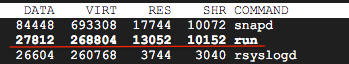
\includegraphics[width=6cm]{images/no_malloc}
	\caption{run without malloc}
    \end{subfigure}
    \hskip2em
    \begin{subfigure}{.4\linewidth}
    	\centering
    	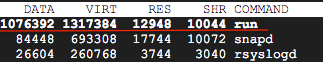
\includegraphics[width=6cm]{images/default_malloc}
	\caption{run with default malloc}
    \end{subfigure}
    \begin{subfigure}{.4\linewidth}
    	\centering
    	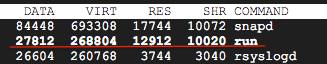
\includegraphics[width=6cm]{images/custom_malloc}
	\caption{run with custom malloc}
    \end{subfigure}
    \hskip2em
    \begin{subfigure}{.4\linewidth}
    	\centering
    	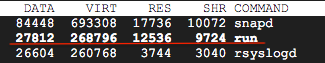
\includegraphics[width=6cm]{images/simple_malloc}
	\caption{run with custom malloc without free}
    \end{subfigure}
    \caption{The Linux top command output for memory usage on 4 different instrumented programs}
    \label{fig:malloc_run}
\end{figure}

\subsection{Performance}

Several different performance tests were carried out in order to measure allocators efficiency in different scenarios. All tests were rerun 100 times with the produced times averaged. Test A allocates 50 chunks of 1kB data and frees it, while Test B allocates 50 different sized (from 1kB to 50kB) chunks of data. Figure \ref{testa_b} shows the times taken to finish tests A and B with the three allocators. The default allocator seems to work very efficiently with single sized data but performed worst on Test B with different sized data. First-fit free-list allocator similarly with both tests, achieving an average of 46.5 \(\mu s\). Allocator without memory re-usage achieved the best times on both tests, averaging 1 \(\mu s\).

\begin{figure}[H]
	\centering
	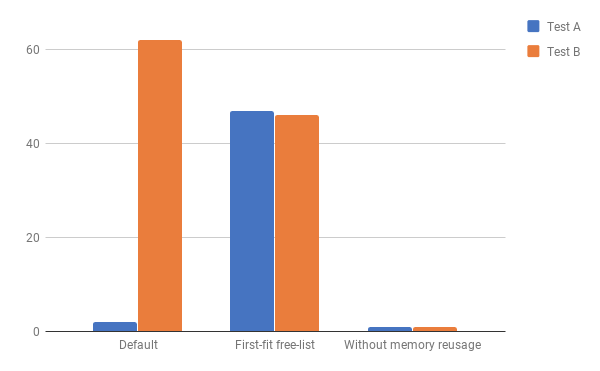
\includegraphics[width=12cm]{allocator_test_a}
	\caption{Test A and B clock time (\(\mu s\)) results for three allocators}
	\label{testa_b}
\end{figure}


Test C allocates a few blocks of 512 bytes of memory, frees them and repeats this loop 10 times. Test D allocates 50 blocks of 1kB data, releases half of it and then allocates and frees memory in a loop. Each test was run twice: once with single size blocks and once with different size blocks. Figure \ref{testc_d} shows the times taken to finish tests C and D with different allocators. Once more the results show that the default allocator is struggling with different size blocks while performing very good with single size blocks. First-fit free-list allocator seems to perform badly on Test D with different size blocks. The poor performance can be explained by one little detail in test D: half of the primarily allocated memory is released by freeing every other block. This means that the first-fit free-list allocator cannot fuse the freed blocks and suffers from fragmentation. On the other hand, the allocator without memory re-usage is again performing outstandingly, averaging 11.5 \(\mu s\) for each test.

\begin{figure}[H]
	\centering
	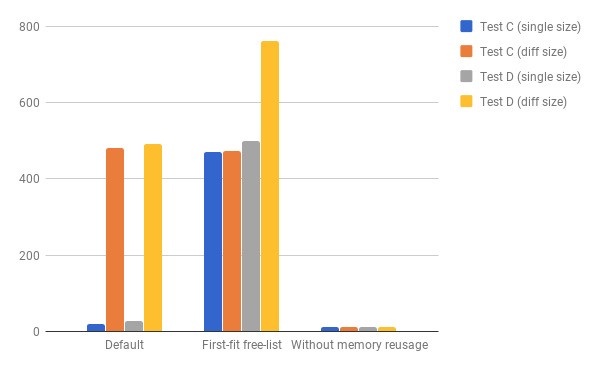
\includegraphics[width=12cm]{allocator_test_c}
	\caption{Test C and D clock time (\(\mu s\)) results for three allocators. Single size means that the test was run with single size blocks, while diff size means that the test was run with different size blocks.}
	\label{testc_d}
\end{figure}

Finally, the last two tests perform tests A and B in parallel. First test A is run with 2 threads, then with 10 threads. The same is done with test B. Figure \ref{teste_f} shows the performance achieved by different allocators during these tests. The default allocator shows quite good times on tests A and B with 2 threads and test A with 10 threads but performs poorly on test B with 10 threads, which confirms the poor performance on different size memory blocks allocation. As explained in Section \ref{consistency} and proven in the chart, synchronisation using locks severely punishes the performance of first-fit free-list allocator, thus it is no surprise it performs worst. The allocator without memory re-usage, however, repeatedly performs best.

\begin{figure}[H]
	\centering
	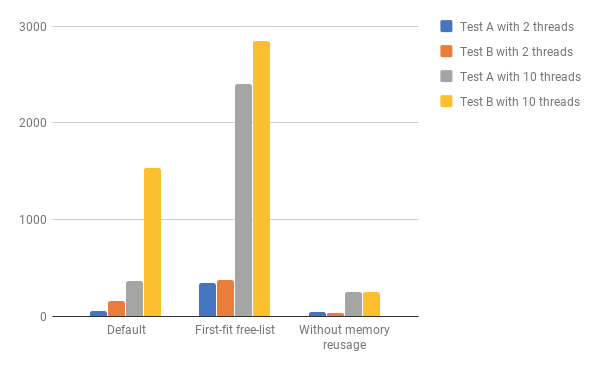
\includegraphics[width=12cm]{allocator_test_e}
	\caption{Test A and B performance results running with 2 and 10 threads.}
	\label{teste_f}
\end{figure}

Overall, the results show that the default allocator works faster than the first-fit free-list allocator but the difference in single-threaded different size block allocations is not tremendous. An allocator without memory re-usage seems to work best and might be a better solution for short running programs.











\chapter{Heap memory translator}
\label{heap-memory-translator}

\section{Motivation}

The translation tool introduced in Chapter \ref{translation-tool} translates all store and load instructions. However, the translated store and load instructions which operate on a stack, BSS or data segments do not actually help save main memory space as the memory for the variables on these segments is still being allocated even though the values are stored on and loaded from cloud storage. This means that only heap memory "translation" gives the desired results and other program memory segments need more complex changes. For instance, BSS and data segments, which consist of initialised and uninitialised static variables, could be stored in cloud storage without allocating space on main memory by implementing a custom compiler frontend. Unfortunately, creating a custom compiler frontend did not seem feasible given the timespan of the project. Instead, a new version of translation tool, which translates only load and store instructions operating on heap memory, was created. The programs translated with the heap memory translator run faster, as it translates only a fraction of the existing store and load instructions. For instance, the tool does not translate such costly variables as loop iterators, which generate vast amounts of load and store instructions in programs.

\section{Implementation}

The easiest way to determine if the variable is stored on the heap is to check if its address is inside the heap address space. If the address of the variable is between the start of the heap and the current break of the heap, then we want to store such variable on the Bigtable. Thus, while iterating through instructions we need to add checks to detect if the address of load or store instruction is inside the heap address space. If it is, we call get or put function on Bigtable and do the similar type casts as in full memory translator. Otherwise, we want to leave the original load or store instruction as is. 

Firstly, the first-fit free-list heap allocator was extended to have two new functions. The getter functions for heap boundaries. In order to accomplish this, the allocator saves the start of the heap on the first call to malloc.

For both store and load instructions the translation starts with calls to get heap boundaries. The address of the instruction, which is being translated, is cast from pointer type to 64-bit integer and compared using \texttt{icmp} instructions with both heap boundaries. The comparison results are conjoined bitwise and used as a condition for a branch instruction. In a case where the bitwise conjunction is equal to 1, the program continues with the instructions for get or put function. Otherwise, the program jumps to the label with the original load or store instructions. If the translated function is load, then a PHI node is added to take on the value corresponding to the input control block (either call to get function or load instruction). PHI node is an instruction used to select a value depending on the predecessor of the current block.

\begin{figure}[H]%
    \centering
    \begin{subfigure}{.45\linewidth}
    	\centering
    	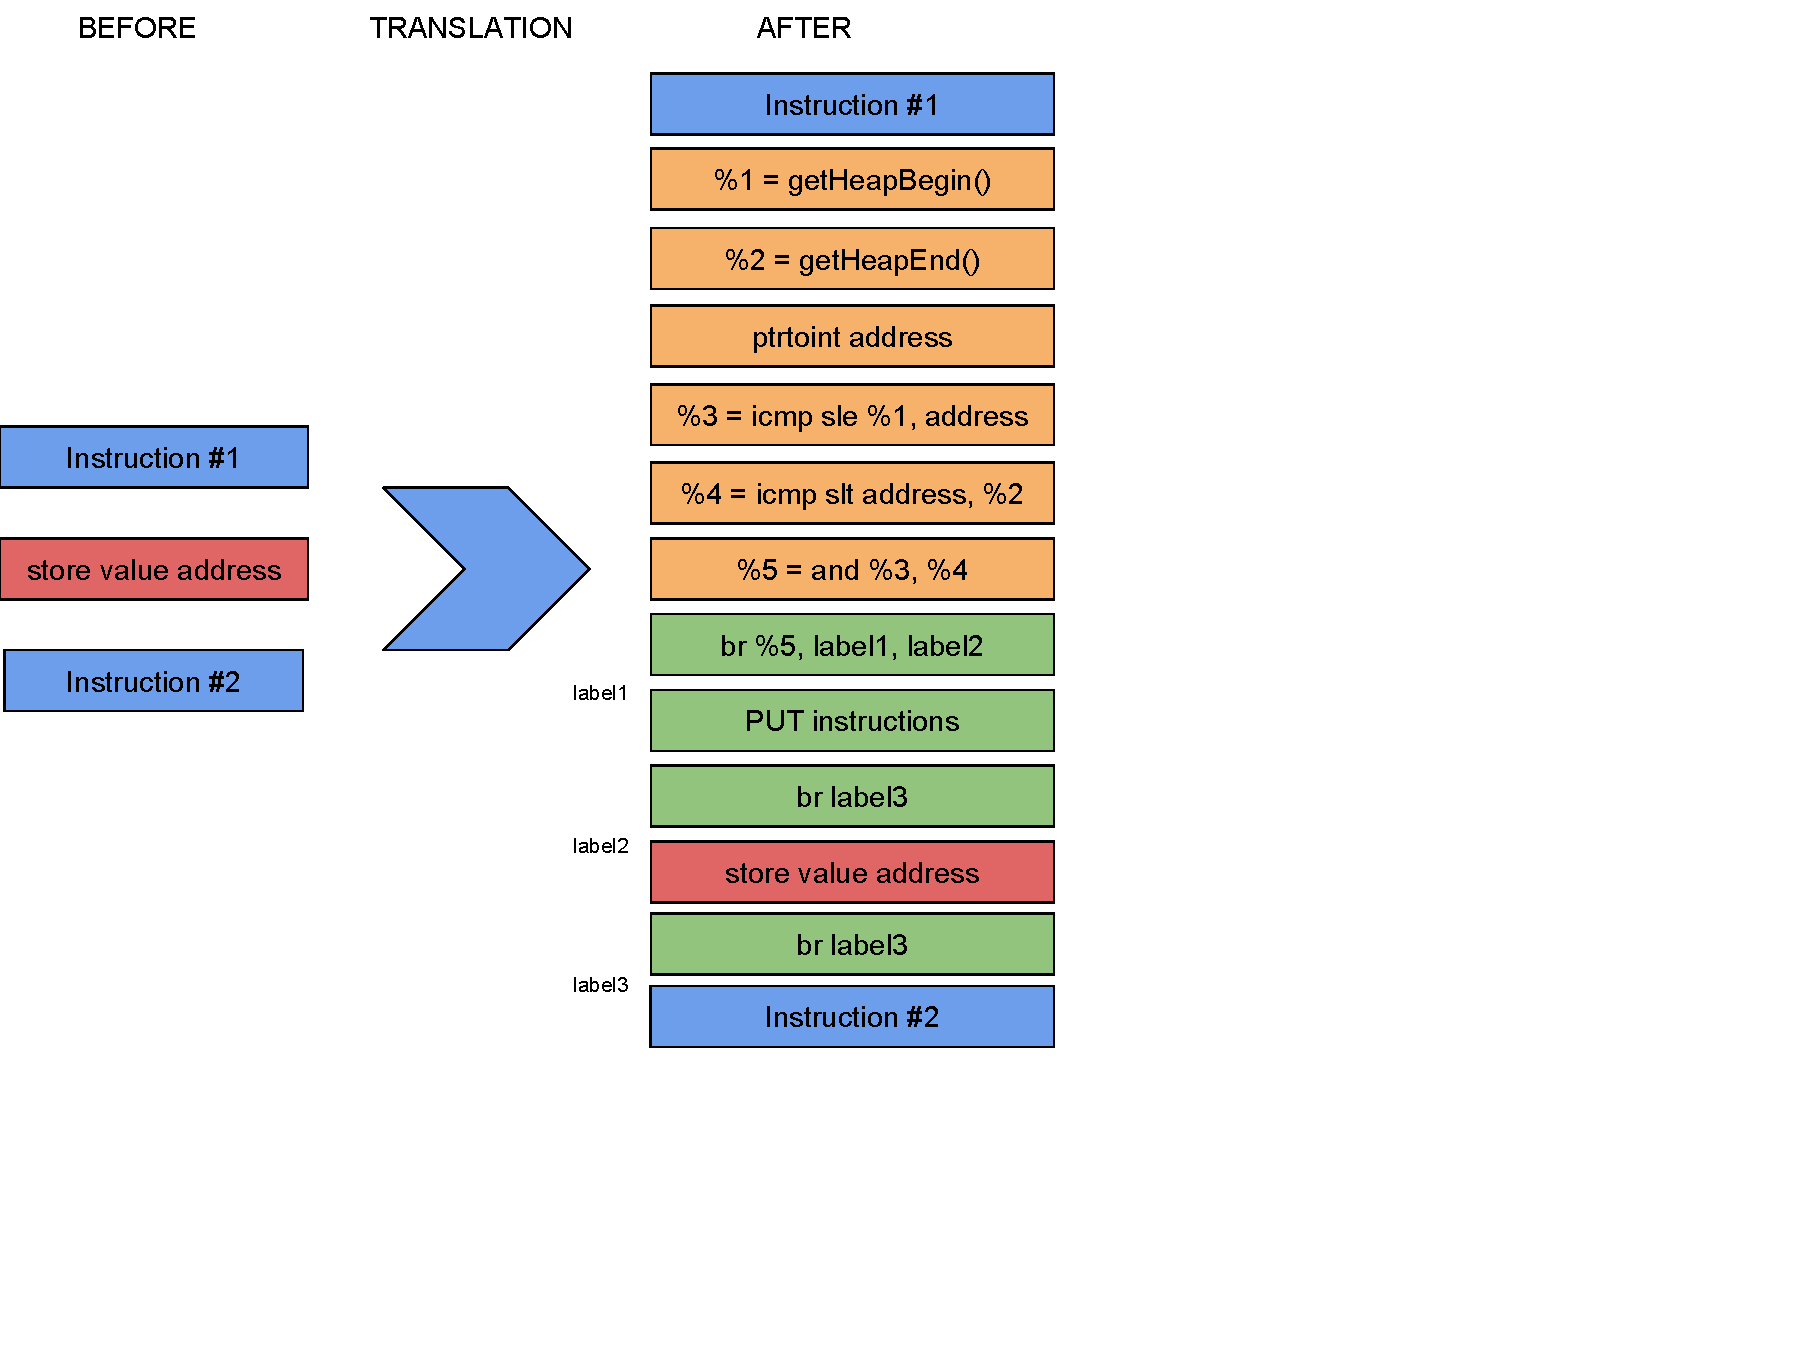
\includegraphics[width=7cm]{images/heap_store_translation}
	\caption{Store instruction translation}
    \end{subfigure}
    \hskip2em
    \begin{subfigure}{.45\linewidth}
    	\centering
    	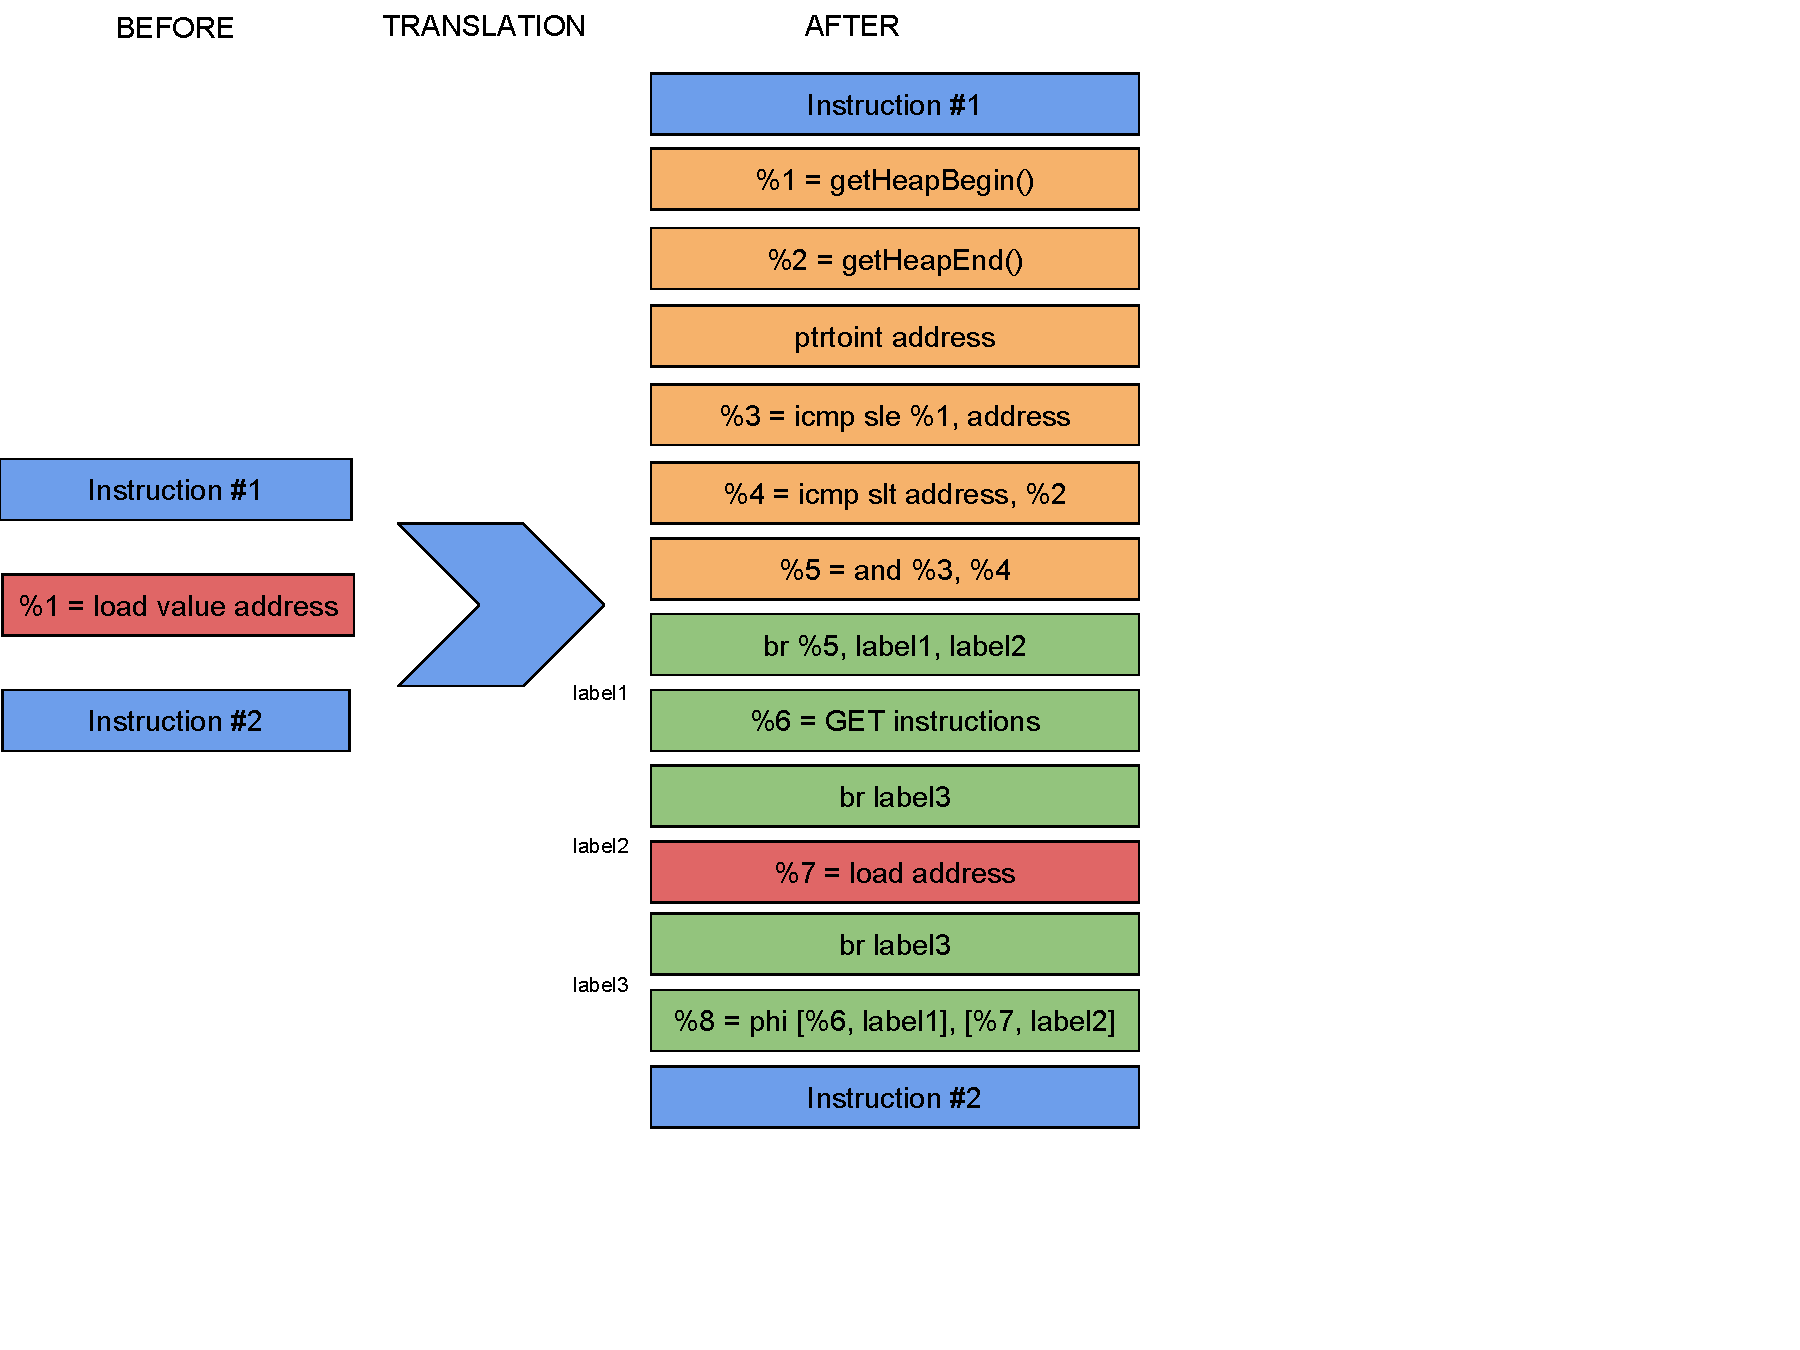
\includegraphics[width=7cm]{images/heap_load_translation}
	\caption{Load instruction translation}
    \end{subfigure}
    \caption{Load and store instruction translation on heap memory translator. Instructions coloured in orange and green are added during the translation.}
    \label{fig:heap_translation}
\end{figure}

As seen in figure \ref{fig:heap_translation}, heap memory translation adds a lot of additional instructions. The insertion of instructions is done in several phases. On the first phase, the first six instructions (coloured in orange) are inserted before the original load or store instruction. Next, the original basic block, the load or store instruction belongs to, is split in two. Between them, two additional basic blocks are created. All this is done using a \texttt{SplitBlockAndInsertIfThenElse} function. After that, the first basic block (label1) is populated by adding a call to get or put function and the casting instructions if needed. The second basic block (label2) is populated with a clone of the original load or store instruction, as the original still exists on the next basic block (label3). Then, the original store instructions are deleted from the last basic block (label3), while the original load instructions are replaced with PHI node instructions. Finally, heap allocator function translations are performed.

\chapter{Evaluation}

Even though the translation tool introduced in this paper does not aim to compete on performance with existing technologies, it is still interesting to compare the original  programs with the ones instrumented with the translation tool. Of course, the efficiency of the system which stores and loads all its memory on another machine, no matter how fast the connection between two machines is, is not going to compete with the system storing and loading memory situated on the same machine. Nonetheless, the performance and other results can be of great value, as they reveal the areas where the tool could be improved.

During the testing and evaluation process, it was decided to measure the performance of individual functions rather than the execution of the whole program itself. This decision was taken in order to exclude the time it takes to load the program into memory and prepare it for execution. These measurements are not affected by the translation tool and are highly depended on the architecture of the machine and the operating system. For the best performance results, the instrumentation tool was tested on Google Compute Engine virtual machine situated on the same data centre as Bigtable instance. 

\section{Performance}

For the performance benchmarking, wall clock time was used instead of CPU time, as it takes into account the time taken for I/O operations (i.e. calls to Bigtable). All tests are run 100 times and averaged, as the execution time of a single test run fluctuates due to external factors (i.e. OS scheduling, memory usage, etc).

The benchmarking was done using three test functions (see Appendix \ref{section:test}), namely stack allocation, heap allocation and parallel producer-consumer problem adapted from Greg Andrews' textbook website \citep{producer-consumer}. The stack allocation test initialises a stack-based 10x10 character matrix with new values. All load and store instructions operate on stack memory. Similarly, the heap allocation test writes values to heap-allocated 10x10 character matrix. Approximately one of ten load and store instructions are for heap-based accesses. Other, stack-based, memory operations are used for iterating through the matrix. The producer-consumer test uses C's POSIX threads (Pthreads) library for thread creation and synchronisation. For this task, the time elapsed includes thread creation and join operations. Two threads were used: one for producer and one for consumer operations. The buffer size was set to 1, while, in total, 50 integers were produced/consumed by the algorithm. The buffer is allocated on the heap in order to have at least one get or put function call when translated with heap translator.

As expected the original program with load and store instructions operating on the main memory of the machine worked efficiently. The producer-consumer took more than a thousand times longer than the other two tests, as the execution time was capped by thread creation and synchronisation time. The stack allocation and heap allocation tests translated with full memory translator took six orders of magnitude longer to execute. This immense increase in time is due to the introduced communication costs to access memory on Bigtable. The producer-consumer problem took half as long to execute, yet the increment from the original code execution time was enormous. Unsurprisingly, the program translated with heap translator showed a huge improvement over the fully translated program in stack allocation test. The improvement is quite clear as none of the load or store instructions are translated, as only heap memory instructions are translated with heap translator. The slow down compared to the original program can be explained by the increase in instruction count of the program (more detailed analysis on this measure provided in the next section). The heap allocation test on the program transformed by heap translator performs 10 times better than the corresponding test instrumented by full memory translator. The test is capped by the time taken to execute 100 put operations with heap memory values on Bigtable. Producer-consumer test again saves some time on load and store instructions on stack variables. The results gathered from benchmarking are shown in table \ref{table:performance}.

\begin{table}[h]
\centering
\begin{tabular}{ c | c c c }
Test & Original & Fully translated & Heap translated \\
\hline
Stack allocation & 0.411 & 2,798,858 & 3 \\
Heap allocation & 0.521 & 2,209,032 & 284,047 \\
Producer-Consumer & 963.717 & 1,272,932 & 295,448
\end{tabular}
\caption{Time taken to execute each function in microseconds ($\mu s$)}
\label{table:performance}
\end{table}

Overall, it can be seen that the heap translation tool is an improvement over full memory translator but it still makes the functions run hundreds (producer-consumer test) and even hundreds of thousands (heap allocation test) times slower than their original counterparts.

\section{Instruction count}

To count the instructions of a program an instruction count pass was implemented. The pass iterates over the functions of the program and prints the count of instructions per function and the total number of instructions in the program. To clarify, this is a static count of the instructions and does not account for how many times any particular instruction can be executed on the runtime. Moreover, the instruction count does not include the instructions from shared library functions. The instruction count pass was run on the test program (see Appendix \ref{section:test}).

\begin{figure}[H]
\centering
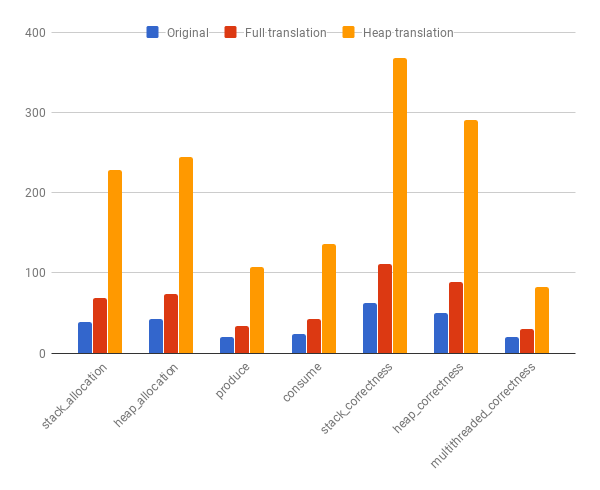
\includegraphics[width=1\textwidth]{images/instruction_count}
\caption{LLVM instruction counts for different functions.}
\label{fig:instruction_count}
\end{figure}

The original program shows the smallest instruction count on every function and works as a baseline for the programs instrumented with the implemented translation tools. The total instruction count for a program translated with full memory translator increased from 571, achieved by the original program, to 761, which shows a 33 percent growth. On average, each function increased by 27 instructions. The inflation is a result of translating one load/store instruction with a call to get/put function instruction plus the additional 1-3 casting instructions. A much more substantial growth can be seen in functions translated by heap memory translator. The total amount of instructions is 209 percent higher than in the original program, increasing from 571 to 1768 instructions. Each function, on average, increased by 171 instructions. This can be explained by the additional control flow added to distinguish between memory access to heap and stack variables. The translation adds 9 to 14 instructions per translated store/load instruction.

Overall, the translation adds a lot of additional instructions. This does not necessarily convert to lower performance of the program (as can be seen by heap translation example with stack allocation test in the previous chapter) and is a much smaller problem then the huge increases in execution time, yet it is definitely a measure which could be improved by additional heuristics.

\chapter{Conclusions}

\section{Overview}

This report has introduced a translation tool (with two of its variations), which provides a way to run programs requiring an amount of memory that cannot be served by user machine. The translation tool instruments the program by changing all load and store instructions to get and put calls on Bigtable, respectively. Additionally, another variation of the translation tool was implemented, which translates only those store and load instructions operating on heap memory. The programs instrumented by heap translation tool run faster than the ones instrumented with full memory translator, as it translates only a fraction of the existing store and load instructions. On the other hand, heap translator significantly increases the number of instructions used in the program. Overall, the report showed that the performance of the instrumented programs are orders of magnitude worse than the original programs, thus there are still lots of things that could be improved.

\section{Future work}

One major area of future work might be to implement a separate front-end compiler. The compiler could make use of the implemented get and put functions when initialising global (static) variables, which in another case would be allocated space on main memory. Somewhat similar (although more complex) strategy could be implemented to prevent stack variables from being allocated space on main memory.

A major performance improvement could be achieved by having the program use main memory and start using Bigtable only when main memory is not enough to serve the requests. One way to achieve this could be incorporating dynamic translation, which would determine when to start to use Bigtable based on some system interrupts indicating lack of memory problem. 

There might also be a way to slightly improve the performance of the translated programs by introducing caches. They would store frequently accessed data on the main memory, thus amortising the communication to Bigtable costs on most frequent values.

Other possible improvements or extensions on the tool:
\begin{itemize}
\item
Find out the source of the thread creation problem mentioned in section \ref{section:other_issues}.
\item
Add support for other LLVM types. For instance, a get and put function overloads should be provided for ConstantFP (floating point) type in order to correctly store floating point values on Bigtable.
\item
Introduce synchronisation through Bigtable between multiple instrumented programs running on different machines. The synchronisation could be achieved by using locks, barriers and other primitives. Bigtable provides an atomic fetch-and-add operation, which can be used as a generalised test-and-set operation, thus making it possible to implement the synchronisation primitives stored there. Combined with cache implementation and an appropriate cache coherence protocol, the updates would let expose Bigtable as distributed shared memory, thus introducing a new usage of the tool.
\end{itemize}

Combined with all these improvements, the translation tool implemented on this project could be a way to solve lack of memory problem or even expose cloud storage as distributed shared memory.

% use the following and \citep{} as above if you use BibTeX
% otherwise generate bibtem entries
\bibliographystyle{plainnat}
\bibliography{mybibfile}

\appendix
\chapter{Test program}
\label{section:test}

\begin{minted}[linenos]{c++}
const int M_X = 10;
const int M_Y = 10;
const int N = 50;
int* target;
int* data;
char *heap_matrix;

void test_stack_allocation(char matrix[][M_Y]) {
  for (int i = 0; i < M_X; i++) {
    for (int j = 0; j < M_Y; j++) {
      matrix[i][j] = (i * M_Y + j) % 128;
    }
  }
}

char *test_heap_allocation() {
  for (int i = 0; i < M_X; i++) {
    for (int j = 0; j < M_Y; j++) {
      *(heap_matrix + i * M_Y + j) = (i * M_Y + j) % 128;
    }
  }
}

void *produce(void *arg) {
  for (int i = 1; i <= N; i++) {
    sem_wait(&empty);
    *data = i;
    sem_post(&full);
  }
  return NULL;
}

void *consume(void *arg) {
  int total = 0;
  for (int i = 0; i < N; i++) {
    sem_wait(&full);
    total += *data;
    sem_post(&empty);
  }
  return NULL;
}

bool test_stack_correctness(char matrix[][M_Y]) {
  for (int i = 0; i < M_X; i++) {
    for (int j = 0; j < M_Y; j++) {
      if (matrix[i][j] != (i * M_Y + j) % 128) {
        cout << i * M_Y + j << "  " << matrix[i][j] << endl;
        return false;
      }
    }
  }
  return true;
}

bool test_heap_correctness(char *matrix) {
  bool correct = true;
  for (int i = 0; i < M_X; i++) {
    for (int j = 0; j < M_Y; j++) {
      if (*(matrix + i * M_Y + j) != (i * M_Y + j) % 128) {
        correct = false;
      }
    }
  }
  free(matrix);
  return correct;
}

void *test_multithreaded_correctness(void *arg) {
  for (int i = 0; i < N; i++) {
    sem_wait(&lock);
    (*target)++;
    sem_post(&lock);
  }
  return NULL;
}
\end{minted}

\end{document}
